\documentclass[leqno, openany]{memoir}
\setulmarginsandblock{3.5cm}{3.5cm}{*}
\setlrmarginsandblock{3cm}{3.5cm}{*}
\checkandfixthelayout

\usepackage{amsmath}
\usepackage{amssymb}
\usepackage{amsthm}
%\usepackage{MnSymbol}
\usepackage{bm}
\usepackage{accents}
\usepackage{mathtools}
\usepackage{tikz}
\usetikzlibrary{calc}
\usetikzlibrary{automata,positioning}
\usepackage{tikz-cd}
\usepackage{forest}
\usepackage{braket} 
\usepackage{listings}
\usepackage{mdframed}
\usepackage{verbatim}
\usepackage{physics}
\usepackage{stmaryrd}
\usepackage{mathrsfs} 
%\usepackage{/home/patrickl/homework/macaulay2}

%font
\usepackage[osf]{mathpazo}
\usepackage{microtype}

%CS packages
\usepackage{algorithmicx}
\usepackage{algpseudocode}
\usepackage{algorithm}

% typeset and bib
\usepackage[english]{babel} 
\usepackage[utf8]{inputenc} 
\usepackage[backend=biber, style=alphabetic]{biblatex}
\usepackage[bookmarks, colorlinks, breaklinks]{hyperref} 
\hypersetup{linkcolor=black,citecolor=black,filecolor=black,urlcolor=black}

% other formatting packages
\usepackage{float}
\usepackage{booktabs}
\usepackage[shortlabels]{enumitem}
\usepackage{csquotes}
\usepackage{titlesec}
\usepackage{titling}
\usepackage{fancyhdr}
\usepackage{lastpage}
\usepackage{parskip}

\usepackage{lipsum}

% delimiters
\DeclarePairedDelimiter{\gen}{\langle}{\rangle}
\DeclarePairedDelimiter{\floor}{\lfloor}{\rfloor}
\DeclarePairedDelimiter{\ceil}{\lceil}{\rceil}


\newtheorem{thm}{Theorem}[section]
\newtheorem{cor}[thm]{Corollary}
\newtheorem{prop}[thm]{Proposition}
\newtheorem{lem}[thm]{Lemma}
\newtheorem{conj}[thm]{Conjecture}
\newtheorem{quest}[thm]{Question}

\theoremstyle{definition}
\newtheorem{defn}[thm]{Definition}
\newtheorem{defns}[thm]{Definitions}
\newtheorem{con}[thm]{Construction}
\newtheorem{exm}[thm]{Example}
\newtheorem{exms}[thm]{Examples}
\newtheorem{notn}[thm]{Notation}
\newtheorem{notns}[thm]{Notations}
\newtheorem{addm}[thm]{Addendum}
\newtheorem{exer}[thm]{Exercise}

\theoremstyle{remark}
\newtheorem{rmk}[thm]{Remark}
\newtheorem{rmks}[thm]{Remarks}
\newtheorem{warn}[thm]{Warning}
\newtheorem{sch}[thm]{Scholium}


% unnumbered theorems
\theoremstyle{plain}
\newtheorem*{thm*}{Theorem}
\newtheorem*{prop*}{Proposition}
\newtheorem*{lem*}{Lemma}
\newtheorem*{cor*}{Corollary}
\newtheorem*{conj*}{Conjecture}

% unnumbered definitions
\theoremstyle{definition}
\newtheorem*{defn*}{Definition}
\newtheorem*{exer*}{Exercise}
\newtheorem*{defns*}{Definitions}
\newtheorem*{con*}{Construction}
\newtheorem*{exm*}{Example}
\newtheorem*{exms*}{Examples}
\newtheorem*{notn*}{Notation}
\newtheorem*{notns*}{Notations}
\newtheorem*{addm*}{Addendum}


\theoremstyle{remark}
\newtheorem*{rmk*}{Remark}

% shortcuts
\newcommand{\Ima}{\mathrm{Im}}
\newcommand{\A}{\mathbb{A}}
\newcommand{\G}{\mathbb{G}}
\newcommand{\N}{\mathbb{N}}
\newcommand{\R}{\mathbb{R}}
\newcommand{\C}{\mathbb{C}}
\newcommand{\Z}{\mathbb{Z}}
\newcommand{\Q}{\mathbb{Q}}
\renewcommand{\k}{\Bbbk}
\renewcommand{\P}{\mathbb{P}}
\newcommand{\M}{\overline{M}}
\newcommand{\g}{\mathfrak{g}}
\newcommand{\h}{\mathfrak{h}}
\newcommand{\n}{\mathfrak{n}}
\renewcommand{\b}{\mathfrak{b}}
\newcommand{\ep}{\varepsilon}
\newcommand*{\dt}[1]{%
   \accentset{\mbox{\Huge\bfseries .}}{#1}}
\renewcommand{\abstractname}{Official Description}
\newcommand{\mc}[1]{\mathcal{#1}}
\newcommand{\msc}[1]{\mathscr{#1}}
\newcommand{\T}{\mathbb{T}}
\newcommand{\mf}[1]{\mathfrak{#1}}
\newcommand{\mr}[1]{\mathrm{#1}}
\newcommand{\ms}[1]{\mathsf{#1}}
\newcommand{\ol}[1]{\overline{#1}}
\newcommand{\ul}[1]{\underline{#1}}
\newcommand{\wt}[1]{\widetilde{#1}}
\newcommand{\wh}[1]{\widehat{#1}}
\renewcommand{\div}{\operatorname{div}}
\newcommand{\bir}{\sim_{\mr{bir}}}

\DeclareMathOperator{\Der}{Der}
\DeclareMathOperator{\Bl}{Bl}
\DeclareMathOperator{\NE}{NE}
\DeclareMathOperator{\Hom}{Hom}
\DeclareMathOperator{\End}{End}
\DeclareMathOperator{\ad}{ad}
\DeclareMathOperator{\Aut}{Aut}
\DeclareMathOperator{\Rad}{Rad}
\DeclareMathOperator{\Pic}{Pic}
\DeclareMathOperator{\supp}{supp}
\DeclareMathOperator{\Supp}{Supp}
\DeclareMathOperator{\sgn}{sgn}
\DeclareMathOperator{\spec}{Spec}
\DeclareMathOperator{\Spec}{Spec}
\DeclareMathOperator{\proj}{Proj}
\DeclareMathOperator{\Proj}{Proj}
\DeclareMathOperator{\ord}{ord}
\DeclareMathOperator{\Div}{Div}

% Section formatting
\titleformat{\section}
    {\Large\sffamily\scshape\bfseries}{\thesection}{1em}{}
\titleformat{\subsection}[runin]
    {\large\sffamily\bfseries}{\thesubsection}{1em}{}
\titleformat{\subsubsection}[runin]{\normalfont\itshape}{\thesubsubsection}{1em}{}

\title{COURSE TITLE}
\author{Lectures by INSTRUCTOR, Notes by NOTETAKER}
\date{SEMESTER}

\newcommand*{\titleSW}
    {\begingroup% Story of Writing
    \raggedleft
    \vspace*{\baselineskip}
    {\Huge\itshape Minimal Model Program Learning Seminar \\ Spring 2021}\\[\baselineskip]
    {\large\itshape Notes by Patrick Lei}\\[0.2\textheight]
    {\Large Lectures by Joaqu\'{\i}n Moraga}\par
    \vfill
    {\Large \sffamily Zoom University}
    \vspace*{\baselineskip}
\endgroup}
\pagestyle{simple}

\chapterstyle{ell}


%\renewcommand{\cftchapterpagefont}{}
\renewcommand\cftchapterfont{\sffamily}
\renewcommand\cftsectionfont{\scshape}
\renewcommand*{\cftchapterleader}{}
\renewcommand*{\cftsectionleader}{}
\renewcommand*{\cftsubsectionleader}{}
\renewcommand*{\cftchapterformatpnum}[1]{~\textbullet~#1}
\renewcommand*{\cftsectionformatpnum}[1]{~\textbullet~#1}
\renewcommand*{\cftsubsectionformatpnum}[1]{~\textbullet~#1}
\renewcommand{\cftchapterafterpnum}{\cftparfillskip}
\renewcommand{\cftsectionafterpnum}{\cftparfillskip}
\renewcommand{\cftsubsectionafterpnum}{\cftparfillskip}
\setrmarg{3.55em plus 1fil}
\setsecnumdepth{subsection}
\maxsecnumdepth{subsection}
\settocdepth{subsection}

\begin{document}
    
\begin{titlingpage}
\titleSW
\end{titlingpage}

\thispagestyle{empty}
\section*{Disclaimer}%
\label{sec:disclaimer}

These notes were taken during the seminar using the \texttt{vimtex} package of the editor \texttt{neovim}. 
Any errors are mine and not the speakers'. 
In addition, my notes are picture-free (but will include commutative diagrams) and are a mix of my mathematical style and that of the lecturers.
If you find any errors, please contact me at \texttt{plei@math.columbia.edu}.

\section*{Acknowledgements}%
\label{sec:acknowledgements}

I would like to thank Joaqu\'{\i}n Moraga for organizing the seminar, finding mistakes in the notes, and more. I would also like to thank Nicol\'as Vilches for providing notes from the times I was unable to attend.

\vspace*{1cm}

\noindent\textbf{Seminar Website:}  \url{https://web.math.princeton.edu/~jmoraga/Learning-Seminar-MMP}
\newpage


\tableofcontents

\chapter{Overview}%
\label{cha:overview}

The goal of the minimal model program is to classify smooth projective complex varieties $X \subseteq \P^n$. Let $T_X$ be the tangent byndle and $\Omega_X$ be the cotangent bundle. Then $\omega_X = \Omega_X^n$ is called the \textit{canonical bundle}, and can be written as $\msc{O}_X(K_X)$ for some Cartier divisor $K_X$.

\begin{quest}
    Can we understand the geometry of $X$ using numerical properties of $K_X$?
\end{quest}

For a curve $C \subseteq X$ and a line bundle $\msc{L}$ on $X$, then $\msc{L}.C = \deg_C(i^* \msc{L})$. Then $K_X$ is \textit{ample (resp. antiample)} if $K_X . C > 0$ (resp $<0$) for all curves $C \subseteq X$. Similarly, $K_X$ is \textit{numerically trivial} if $K_X . C = 0$ for all curves $C \subseteq X$.

\begin{defn}
    We say that $X$ is \textit{Fano} if $K_X$ is antiample, \textit{Calabi-Yau} if $K_X$ is numerically trivial, and \textit{canonically polarized} if $K_X$ is ample.
\end{defn}

\begin{exm}
    If $C$ is a Fano curve, then $C \simeq \P^1$. If $C$ is a CY curve, then $C$ is an elliptic curve. If $C$ is a canonically polarized curve, then $g(C) \geq 2$.
\end{exm}

\begin{exm}
    Let $X \subseteq \P^n$ be a smooth hypersurface of degree $d$. Then by the adjunction formula, we have $K_X \simeq \eval{(K_{\P^n} + X)}_X \simeq \eval{(d-n-1)H}$. Therefore, $X$ is Fano if $d \leq N$, CY if $d = n+1$, and canonically polarized if $d \geq n+2$.
\end{exm}

\begin{rmk}
    If $E$ is an elliptic curve, then $E \times \P^1$ has $K_X . C = 0$ for some curves and $K_X . C < 0$ for others.
\end{rmk}

Now we consider various properties of different varieties:
\begin{table}[H]
    \centering
    \caption{Properties of varieties of different classes}
    \label{tab:label}
    \begin{tabular}{rlcl}
    \toprule
    & Fano & CY & Canonically polarized \\
    \midrule
        $\pi_1$ & trivial & {?} & generally infinite \\
        Automorphisms & linear algebraic groups & {?} & finite groups \\
        Birational automorphisms & monstrous & {?} & finite groups \\
        Geometry & simple geometry & {?} & complicated, rich \\
        Arithmetic & a lot of $\Q$-points & {?} & $\Q$-points in a proper closed \\
        \bottomrule
    \end{tabular}
\end{table}
We have said nothing about Calabi-Yaus, but of course by the Beauville-Bogomolov decomposition, we can reduce to pure Calabi-Yaus ($h^{i,0} = 0$ for $0 < i < \dim X$), hyperk\"ahlers, and abelian varieties up to taking a finite cover.

Now let $x$ be a closed point on $X$. Then there is a variety $\Bl_x X \to X$ that is an isomorphism away from $x$ where the fiber above $x$ is an exceptional divisor $E$ parameterizing tangent directions at $x$.

\begin{exm}
    Consider points $p_1, \ldots, p_n, \ldots \in \P^2$. Then if we blow up these points in a sequence, we obtain a sequence of varieties $X_1, \ldots, X_2, \ldots, X_n, \ldots$ Over $\P^2 \setminus \qty{p_1, \ldots, p_{i-1}}$, the morphism $X_i \to \P^2$ is an isomorphism. For $i \neq j$, clearly $X_i$ is not isomorphic to $X_j$ (they have different Picard ranks), but they are \textit{birational}. We say that $X_1 \bir X_2$ if they have isomorphic dense open subsets.
\end{exm}

Now we can state the goal of the Minimal Model Program. If $X$ is projective and has ``mild singularities'' the goal is to prove that there exists a birational map $\pi \colon X \dashrightarrow X'$ and a fibration ($\varphi_* \msc{O}_{X'} = \msc{O}_Z$ and positive dimensional general fiber) $X' \xrightarrow{\varphi} Z$ such that one of the following holds:
\begin{enumerate}
    \item $F$ is Fano;
    \item $F$ is Calabi-Yau;
    \item $Z = \Spec \C$ and $X'$ is canonically polarized.
\end{enumerate}
The way we will construct this birational morphism is by studying the geometry of curves on $X$ which intersect $K_X$ negatively. If $K_X.C < 0$ under some hypotheses (extremity on $NE(X)$), we can find $\varphi_C \colon X \to X_1$ contracting precisely the curves which are numerically equivalent to a positive multiple of $C$.

\begin{enumerate}
    \item If the curves numerically equivalent to a positive multiple of $C$ cover $X$, then $\varphi_C$ has positive-dimensional fibers, is a contraction, and the general fiber $F$ is Fano. This is called a \textit{Mori fiber space}.
    \item If the curves numerically equivalent to a positive multiple of $C$ cover a divisor on $X$, then we say that $\varphi_C \colon X \to X_1$ is a divisorial contraction and thus $\rho(X_1) = \rho(X) - 1$. $X_1$ still has nice singularities, so we can iterate this process.
    \item The last case is called a small contraction. The curves which are numerically equivalent to a positive multiple of $C$ cover a set of codimension at least $2$. In this case, $X_1$ may have very bad singularities (by this, we mean that $K_{X_1}$ is not $\Q$-Cartier). We construct a new birational morphism $\varphi_C^+ \colon X^+ \to X_1$ which contracts $K_{X^+}$-positive curves.
\end{enumerate}

Another type of surgery is a flip, which changes a locus of codimension at least $2$. For example, consider $D = p_1^* \msc{O}(1) \otimes p_2^* \msc{O}(r)$ on $\P^1 \times \P^1$. Then write
\[ X = \Spec \qty(\bigoplus_{m \geq 0} H^0 (\P^1 \times \P^1, \msc{O}_{\P^1 \times \P^1}(mD))). \]
Then $X$ is (locally) a cone over $\P^1 \times \P^1$, so $K_X$ is not $\Q$-Cartier. Therefore, we can blow up the vertex, and the exceptional divisor is $E \simeq \P^1 \times \P^1$. Now the $\P^1 \times \P^1$ can be collapsed onto each of the two factors, so we obtain a birational map $\pi \colon X_1 \dashrightarrow X_1^+$. Here, if $C,C^+$ are the resulting curves, we have $K_{X_1}.C < 0$ and $K_{X_1^+}.C^+ > 0$.
\begin{figure}[H]
    \centering
    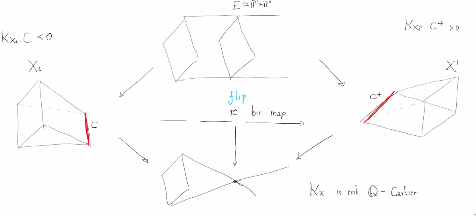
\includegraphics[width=0.8\linewidth]{flip}
    \caption{A Flip}%
    \label{fig:flip}
\end{figure}
This gives us the question:
\begin{quest}
    Do flips always exist?
\end{quest}
Now either the algorithm given by iterating this process always terminates or it continues infinitely. We are fine once we reach the Mori fiber space case, and there are only $\rho(X) - 1$ divisorial contractions, so the only possible problem is that there is an infinite sequence of flips.

\begin{conj}[Termination of flips]
    This algorithm always terminates after finitely many flips with either a Mori fiber space $X_n \to Z$ or a variety $X_n$ such that $K_{X_n}.C \geq 0$ for every curve $C$ (in other words, $K_{X_n}$ is nef).
\end{conj}

\begin{conj}[Abundance]
    $X$ has mild singularities and $K_X$ is nef. Then $\abs{m K_X}$ is basepoint-free for some $m \gg 0$.
\end{conj}

If this is true, and $X \xrightarrow{\varphi} X_1$ contracts all $K_X$-trivial curves, then either
\begin{enumerate}
    \item The general fiber has positive dimension. In this case, $K_F \equiv 0$.
    \item $\dim X = \dim X_1$. Then $X \to X_1$ is birational and $X_1$ is canonically polarized.
\end{enumerate}

Therefore, the goal of the MMP is achieved if we can solve the conjectures of existence of flips, termination of flips, and abundance. Existence of flips was proved by Birkar, Cascini, Hacon, and McKernan in 2006 and termination is known in dimension at most $3$ and in some cases in dimension $4$. Finally, abundance is known in dimension at most $3$.

\chapter{MMP in Dimension $3$}%
\label{cha:mmp_in_dimension_3_}

\section{Rational Curves}%
\label{sec:bend_and_break}

\begin{prop}[Bend and Break]
    Let $X$ be proper and $C$ be a smooth proper curve. Let $p \in C$ and $g_0 \colon C \to X$ be nonconstant. Next, let $0 \in D$ be a pointed curve and $G \colon C \times D \to X$ such that
    \begin{enumerate}
        \item $\eval{G}_{C \times \qty{0}} = g_0$.
        \item $G(\qty{p} \times D) = g_0(p)$.
        \item $\eval{G}_{C \times \qty{t}}$ is different from $g_0$ for general $t$.
    \end{enumerate}
    All of these imply that this is a nontrivial deformation of $g_0$ fixing $p$. Then there exists $g_1 \colon C \to X$ and $Z = \sum a_i Z_i$ a union of rational curves such that ${(g_0)}_* C$ is algebraically equivalent to ${(g_1)}_* (C) + Z$ and $g_0(p) \in \bigcup_i Z_i$. In particular, there exists a rational curve through $g_0(p)$.
\end{prop}

\begin{proof}
    First, compactify $D$ and let $\ol{G} \colon C \times \ol{D} \dashrightarrow X$ be the rational map. This map is undefined at $\qty{p} \times \ol{D}$ by the rigidity lemma, so let $S$ be the normalization of the graph of $\ol{G}$. So we have a map $\pi \colon S \to C \times \ol{D}$ and write $G_S \colon S \to $. 

    Then we define $h \colon S \to C \times \ol{D} \to \ol{D}$. Then there exist $d \in C \times \ol{D}$ such that $\pi$ is not an isomorphism over $d$. Then we know that $h^{-1}(d) = C' + E$ where $C'$ is a birational transform of $C$ and $E$ is $\pi$-exceptional. Then we set $g_1 \colon C \to X$ to be the restriction of $G_S$ to $C'$ and $Z = G_S(E)$.

    By a lemma of Abhyankar, we know that $E$ is a union of rational curves, and then by the L\"uroth theorem, we know that $Z$ is a union of rational curves and
    \[ {(g_0)}_* C \sim_{\mr{alg}} {(g_1)}_* C + Z. \]
\end{proof}

\begin{lem}[Abhyankar]
    Let $X$ have mild singularities and $Y \xrightarrow{\pi} X$ be a proper birational morphism. For any $x \in X$, either $\pi^{-1}(x)$ is a point or is covered by rational curves.
\end{lem}

Here is an intuitive image of the bend-and-break process:
\begin{figure}[H]
    \centering
    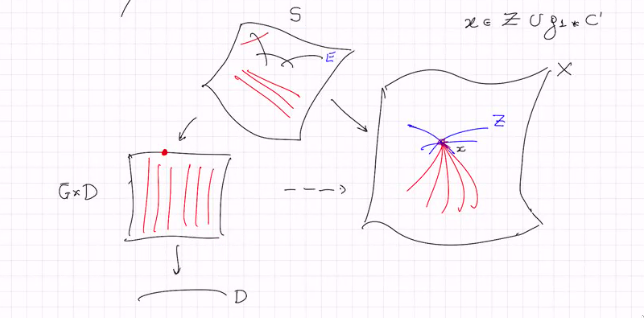
\includegraphics[width=0.8\linewidth]{bendbreak}
    \caption{Bend and Break}%
    \label{fig:bendbreak}
\end{figure}

\begin{prop}[Bend and Break II]
    Let $X$ be a projective variety and $g_0 \colon \P^1 \to X$ be a nonconstant morphism. Let $D$ be a smooth pointed curve and $G \colon \P^1 \times D \to X$ such that
    \begin{enumerate}
        \item $\eval{G}_{\P^1 \times \qty{0_D}} = g_0$;
        \item $G(\qty{0} \times D) = g_0(0), G(\qty{\infty} \times D) = g_0(\infty)$;
        \item $G(\P^1 \times D)$ is a surface.
    \end{enumerate}
    Then ${(g_0)}_* \P^1$ is algebraically equivalent either to a reducible curve or a multiple curve.
\end{prop}

\begin{proof}
    Let $S$ be a $\P^1$-bundle containing $\P^1 \times D$ and consider the rational map $\wt{G} \colon S \dashrightarrow X$. Then we can resolve the basepoints to obtain $\wt{G} \colon \wt{S} \to S$ and induct on $\rho(\wt{S} / S) \eqqcolon \rho$.
    \begin{description}
        \item[Case 1: $\rho = 0$:] Consider the sections $C_0, C_{\infty}$ at $0$ and $\infty$. Then let $H$ is ample on $X$ and then we see that ${(\wt{G}^* H)}^2 > 0$ and ${(C_0 \cdot \wt{G}^* H)} = {(C_{\infty} \cdot \wt{G}^* H)} = 0$ by the projection formula. By the Hodge index theorem, we see that $C_0^2 < 0, C_{\infty}^2 < 0$ (because $\wt{G}^* H, C_0, C_{\infty}$ are linearly independent). But then we know that $\rho(S) = 2$, which is a contradiction.
        \item[Inductive step:] Consider the diagram
            \begin{equation*}
            \begin{tikzcd}
                \wt{S} \ar{rr}{\wt{G}} \ar{d}{r'} \ar[swap,bend right=40]{dd}{\wt{r}} & & X \\
                S' \ar{d}{r} \ar[dashrightarrow]{urr}{\ol{G}'} \\
                S \ar{d}{q} \ar[swap,dashrightarrow]{uurr}{\ol{G}} \\
                D.
            \end{tikzcd}
            \end{equation*}
            Then $r$ is the first blowup in $\wt{S} \to S \ni P$ and $y \in D$ will be a point such that $P \in q^{-1}(y)$. Let $F_1$ be the exceptional divisor of $r$ and $F_2$ be the strict transform of $q^{-1}(y)$ in $S'$. Then $F_1, F_2$ intersect at a point $Q$. But then $\ol{G}'$ is a morphism around $F_2$. But then ${(g_0)}_* \P^1 \sim \wt{G}_* ({(q \circ r)}^* (y))$, which is reduced and irreducible. If $\ol{G}$ is not defined at $Q \neq P$, then
            \[ \wt{G}_* ({(q \circ r)}^* (y)) = \wt{G}_* \mr{red}(\wt{r}^{-1}(p)) + \wt{G}_* \mr{red} (\wt{r}^{-1}(Q)) + (\text{effective}), \]
            which is a contradiction and thus $\ol{G}$ is defined at $Q \neq P$. Then if $\ol{G}'$ is not defined at $Q_0$, then after blowing up $Q_0$, we see that ${(q \circ r)}^* (y)$ must contain a component of multiplicity at least $2$. Now contracting $F_2$, we have the desired result by induction on $\rho$. \qedhere
    \end{description}
\end{proof}

This tells us that to produce rational curves, we simply need to deform them with enough fixed points and use bend and break. But now we need to actually find rational curves.

\begin{thm}
    Let $X$ be smooth and projective and $-K_X$ be ample. For every $x \in X$, there exists a rational curve $C$ through $x$ such that
    \[ 0 < -K_X . C \leq \dim X + 1. \]
\end{thm}

\begin{proof}
    Choose some curve $C \subseteq X$ through $x$. Then the space of deformations of $C$ on $X$ fixing $x$ has dimension at least
    \[ h^0(C, f^* T_X) - h^1(C, f^* T_X) - \dim X = - f_* C. K_X - g(C) \dim X. \]
    We have several cases:
    \begin{enumerate}
        \item If $g(C) = 0$, then we are done.
        \item If $g(C) = 1$, then we can replace $f$ with the composition by an endomorphism of large degree $n$, then we see that
            \[ - ({(f \circ h)}_* C \cdot K_X) - \dim X = -n^2 f_* C.K_X - \dim X > 0 \]
            whenever $n$ is sufficiently large
        \item Assume $g(C) \geq 2$. Then there are no endomorphisms of high degree, so assume $X, C$ are defined over $\Z$. Then let $X_p, C_p$ be the reduction to $\ol{F}_p$. Now we apply the Frobenius map $F_p$, which has degree $p$. By generic flatness, we know that ${(f_p)}_* C_p.K_{X_p}, g(C_p), \chi\qty(\eval{T_X}_{C_p})$ are the same for almost all $p$, so by the same argument as in the genus $1$ case, we see have a rational curve $A_p$ on $X_p$ for almost all $p$. By bend and break II, we can find a rational curve of the desired degree.

            Then we use the fact that if a statement holds for all $p$ large enough, then it holds for the complex numbers, and we obtain a curve. This is analogous to the idea that if $Z \subseteq \P^n_{\Z}$, then if the image of $\pi \colon Z \to \Spec \Z$ contains a Zariski-dense subset, then it contains the generic point. \qedhere
    \end{enumerate}
\end{proof}

\begin{thm}
    Let $X$ be a smooth projective variety and let $H$ be ample on $X$. Assume there exists $C' \subseteq X$ such that $-(C'.K_X) > 0$. Then there exists a rational curve $E$ such that $\dim X + 1 \geq -(E.K_X) > 0$ and
    \[ \frac{-(E.K_X)}{E.H} \geq \frac{-C'.K_X}{C'.H}. \]
\end{thm}

\begin{thm}[Cone Theorem]
    Let $X$ be smooth and projective. Then there exist countably many curves $C_r \subseteq X$ such that $0 < - K_X.C_i \leq \dim X + 1$ and 
    \[ \ol{\NE}(X) - {\ol{\NE}(X)}_{K_X \geq 0} + \sum_i \R_{\geq 0} [C_i]. \]
\end{thm}

\begin{proof}
    Choose $C_i$ with $0 < -(C.K_X) \leq \dim X + 1$ and let $W$ be the closure of $\ol{\NE}_{K \geq 0} + \sum_i \R_{\geq 0} [C_i]$. Now choose $D$ positive on $W \setminus \qty{0}$ and negative somewhere on $\ol{\NE}(X)$. Let $H$ be ample and 
    \[ \mu = \max \qty{\mu' \mid H + \mu' D\ \text{is nef}}. \] 
    This means that $H + \mu D$ is nef. Then let $Z \in \ol{\NE}(X)$ with $(H+\mu D).Z = 0$ and $K_X.D < 0$. Let $Z_k$ be a sequence of curves approximating $Z$. Then we see that
    \[ \max_j \frac{- (Z_{k_j}. K_X)}{(Z_{k_j}.(H + \mu'D))} \geq \frac{-Z_k.K_X}{Z_k.(H+\mu D)} \]
    is obtained by $Z_{k_0}$. Now we will replace $Z_k$ with rational curves $E_{i(k)}$ such that $\dim X + 1 \geq - E_{i(k)}.K_X > 0$ and 
    \[ \frac{-E_{i(k)}.K_X}{E_{i(k)}.(H + \mu' D)} \geq \frac{-Z_{k_0}.K_X}{Z_{k_0}.(H+\mu'D)} \geq \frac{-Z_k.K_X}{Z_k.(H+\mu'D)}. \]
    Because $E_{i(k)}.D \geq 0$, we have
    \[ \frac{-E_{i(k)}.K_X}{E_{i(k)}.H} \geq \frac{-Z_k.K_X}{Z_k.(H+\mu'D)}. \]
    Fixing $M \gg 0$ such that $MH + K_X$ is ample, then we see that $(MH + K_X).E_{i(k)} > 0$, so
    \[ M > \frac{- E_{i(k)}.K_X}{E_{i(k)}.H} \geq \frac{-Z_k.K_X}{Z_k.(H+\mu'D)}. \]
    Taking $k \to \infty, \mu' \to \mu$, we see that
    \[ M > \frac{Z.K_X}{Z.(H+\mu D)} \longrightarrow \infty, \]
    a contradiction.
\end{proof}

\begin{exm}
    Suppose $K_X$ is not nef. Then there are no rational curves on $X$. For example, there are no rational curves of an abelian variety.
\end{exm}

\section{Singularities of the MMP}%
\label{sec:singularities_of_the_mmp}

Consider pairs $(X, \Delta)$ such that $X$ is normal quasiprojective and $K_X + \Delta$ is $\Q$-Cartier. These are called \textit{log pairs}. 

\begin{defn}
    Let $\pi \colon Y \to X$ is a resolution of singularities, $E \subseteq Y$ is exceptional, and $\pi^* (K_X + D) + \sum E_i$ has simple normal crossings. Define the \textit{log discrepancy} 
    \[ a_E(X, D) \coloneqq 1 + \operatorname{coeff}_E (K_Y - \pi^* (K_X + D)). \]
\end{defn}

\begin{defn}
    We say that $(X, \Delta)$ is 
    \begin{enumerate}
        \item \textit{terminal} if $a_E(X, \Delta) > 1$ for every exceptional $E$ over $Y$.
        \item \textit{canonical} if $a_E(X, \Delta) \geq 1$ for every exceptional $E$ over $Y$.
        \item \textit{Kawamata log terminal} if $a_E(X, \Delta) > 0$ for every $E$.
        \item \textit{log canonical} if $a_E(X, \Delta) \geq 0$ for every $E$.
    \end{enumerate}
\end{defn}

Now if $X$ is smooth projective and $K_X$ is pseudoeffective, then there exists $X \dashrightarrow X_{\mr{ter}}$ such that $K_{X_{\mr{ter}}}$ is nef. By abundance, $K_{X_{\mr{ter}}}$ is semiample. Then there is a morphism $X_{\mr{ter}} \to X_{\mf{can}}$ such that $K_{X_{\mr{can}}}$ is ample. Then terminal singularities are those that may appear in the terminal model, and canonical singularities are those that may appear on the canonical model.

Recall the \textit{adjunction formula}: If $(X, D)$ is log smooth, then $K_X + \eval{D}_D \sim K_X$. Usually, $(X,D)$ is log canonical but not klt. But then $a_D(X,D) = 0$ but $a_E(X, D) > 0$ for every $E \neq D$. Terminal singularities are the smallest category of singularities that we need to understand to run the minimal model program. On the other hand, log canonical is the largest class of singularities in which we can expect the MMP to work.

\begin{exm}[Examples of klt singularities]
    Both cone singularities and quotient singularities are klt. 
\end{exm}

\begin{prop}[Cones]
    Let $(X, \Delta)$ be a log pair and $A$ an ample Cartier divisor on $X$. Then define
    \[ C(X, \Delta) = \Spec (\bigoplus_{m \geq 0} H^0(X, \msc{O}_X(mA))). \]
    Then $C(X, A)$ is 
    \begin{enumerate}
        \item terminal if and only if $rA \sim_{\Q} K_X + \Delta$ with $r < -1$ and $(X, \Delta)$ terminal;
        \item canonical if and only if $ra \sim_{\Q} k_x + \delta$ with $r \leq -1$ and $(X, \Delta)$ canonical;
        \item klt if and only if $ra \sim_{\Q} k_x + \delta$ with $r < 0$ and $(X, \Delta)$ is klt;
        \item log canonical if and only if $ra \sim_{\Q} k_x + \delta$ with $r \leq 0$ and $(X, \Delta)$ is log canonical.
    \end{enumerate}
    In particular, the cone over a Fano is klt, the cone over a Calaby-Yau is log canonical, and cones over canonically polarized varieties are terrible.
\end{prop}

\begin{exm}
    Consider the cone $C_n$ over a rational normal curve of degree $n$. Then resolving $Y_n \to C_n$, we see that the exceptional $E_n \simeq \P^1$ and 
    \[ \pi^* (K_{C_n}) = K_{Y_n} + \qty(1 - \frac{2}{n}) E_n, \] 
    and therefore $a_{E_n}(C_n) = \frac{2}{n}$.

    Consider $E \subseteq \P^3$ and elliptic curve. Then $\pi^*(K_{C_E}) = K_{Y_E} + E$, so $a_E(C_E) = 0$.
\end{exm}

Now consider $G \subseteq GL_n$ a finite group. Then $\C^n/G = \Spec {\C[x_1, \ldots, x_n]}^G$ has klt singularities.

\begin{exm}
    In dimension $2$, we have
    \begin{enumerate}
        \item terminal is equivalent to smooth;
        \item canonical is equivalent to ADE;\@
        \item klt is equivalent to quotient singularity;
        \item log canonical is ``equivalent'' to quotient and/or elliptic cone.
    \end{enumerate}
\end{exm}

\begin{exm}
    In dimension $3$, terminal singularities are classified as quotients of hypersurface singularities, also known as \textit{hyperquotient singularities}. Then are given by actions of finite groups $G$ acting on hypersurface singularities of the form $\qty{x^2 + y^2 + f(z, w) = 0}$. Even for canonical singularities, we have no idea what they look like.
\end{exm}

\begin{exm}
    In dimension $4$, there are examples of $4$-fold terminal singularities with analytic embedding dimension $n$ for every $n$ (Kollar, 2010). By contrast, terminal singularities in dimension $3$ all have analytic embedding dimension $4$.
\end{exm}

\begin{thm}[Prokhorov, Xu, 2019]
    Any klt singularity deforms to a klt cone singularity. For $x \in X$, there exists a flat morphism $\msc{X} \xrightarrow{\varphi} \A^1$ such that $\varphi(\A^1 \setminus 0) \sim (\A^1 \setminus 0) \times X$ and $\varphi^{-1}(0) = X_0$ is a klt cone singularity. This is just a deformation to the normal cone.
\end{thm}

We will apply the following philosophy: 
\begin{quotation}
    \textit{Any theorem for smooth projective varieties should work with klt singularities}. 
\end{quotation}

\begin{exm}
    Let $K_X = 0$. By Beauville-Bogomolov (1970s), there exists a cover $X \gets Y$, where $Y$ is a product of abelian varieties, irreducible Calabi-Yau varieties, and hyperk\"ahlers. There is an analogue for klt singularities that was proved by Druel, Campana,\ldots in 2020.
\end{exm}

\begin{exm}
    Let $X$ be smooth projective and $-K_X$ be nef. Then 
    \[ \wt{X} \sim \C^q \times \prod Y_i \times \prod S_k \times Z, \]
    where $Y_i$ is strict Calabi-Yau, $S_k$ is hyperkahler, and $Z$ is rationally connected. There is a version for klt singularities in progress.
\end{exm}

We will now discuss localization of singularities. Suppose $X$ is a variety with terminal singularities and $Z \subseteq X$ a subvariety of codimension $1$. Then $\Spec \msc{O}_{X,Z}$ has terminal singularities if and only if $\Spec \msc{O}_{X,Z}$ is a smooth local ring, and this is equivalent to smoothness at the generic point of $Z$. In particular, if $X$ is terminal, the singularities must appear in codimension at least $3$.

\section{Vanishing}%
\label{sec:vanishing}

Let $C \subseteq X$ be a $K_X$-negative curve. Then if $K_X \sim_{\Q} E \geq 0$ for some $E$ effective, we see that $K_X.C = E.C < -$, so $C \subseteq E$. Now if $(X, D)$ is a log smooth pair, we have an exact sequence
\[ 0 \to \msc{O}_X(K_X) \xrightarrow{\otimes D} \msc{O}_X (K_X \times D) \to \msc{O}_D(K_D) \to 0. \]
If $H^1(X, \msc{O}_X(K_X)) = 0$, then $H^0(K_X + D) \twoheadrightarrow H^0(K_D)$. This tells us that vanishing theorems help us find sections of line bundles.

\begin{thm}[Kodaira Vanishing]
    Let $X$ be smooth projective and $\msc{L}$ be ample. Then $H^i(X, \msc{L}^{-1}) = 0$ for all $i < \dim X$.
\end{thm}

\begin{proof}[Sketch of Proof]
    Let $s \in H^0(X, \msc{L}^m)$ and $D = (s=0)$ be smooth. Then we have $\msc{O}_X \xrightarrow{s} \msc{L}^m$. Now we have
    \[ \msc{L}^{-i} \otimes \msc{L}^{-j} \simeq \msc{L}^{-i-k} \msc{O}_X \xrightarrow{\mr{id} \otimes s} \msc{L}^{-i-j} \otimes \msc{L}^m = \msc{L}^{-i-j+m}. \]
    Setting $Z = \Spec \bigoplus_{i=0}^{m-1} \msc{L}^{-i}$ with projection $p \colon Z \to X$, we note that if $X, D$ are smooth, then $Z$ is smooth. Consider a morphism $\tau \colon H^i(Z, \C_Z) \twoheadrightarrow H^i(Z, \msc{O}_Z)$ and its pushforward $p_* \tau \colon H^i(X, p^* \msc{C}_Z) \twoheadrightarrow H^i(X, p_* \msc{O}_Z)$. Now we consider the surjection
    \[ \bigoplus_{r=0}^{m-1} H^i(X, \C[\zeta^r]) \twoheadrightarrow \sum_{r=0}^{m-1} H^i\qty(X, \bigoplus_{r=0}^{m-1} \msc{L}^{-r}). \]
    Now we use the result that $\C[\zeta^r] \hookrightarrow \msc{L}^{-r}$ factors through $\C[\zeta^r] \hookrightarrow \msc{L}^{-r}(-k D) \hookrightarrow \msc{L}^{-r}$. By Serre, we see that $H^i(X, \msc{L}^{-(r+mk)}) = 0$ for arbitrary $k$.
\end{proof}

\begin{thm}[KV vanishing]
    Let $X$ be a smooth projective complex and $\msc{L}$ be a line bundle on $X$ such that $\msc{L} \equiv M + \sum a_i D_i$, where $M$ is a big and nef $\Q$-divisor, $\sum D_i$ is a snc divisor, and $0 \leq a_i < 1, a_i \in \Z$. Then $H^i(X, \msc{L}^{-1}) = 0$ for $i < \dim X$.
\end{thm}

\begin{prop}
    Let $X$ be quasiprojective and normal, $D$ Cartier, and $m > 0$ a positive integer. Suppose $Y \xrightarrow{p} X$ is finite and $D'$ Cartier such that $p^* D \sim MD'$. If $X$ is smooth and $\sum F_j$ is simple normal crossing, then $Y$ is smooth and $\sum p^* F_j$ has simple normal crossings.
\end{prop}

\begin{lem}
    Let $Y \to X$ be finite. Then $\msc{O}_X \to f_* \msc{O}_Y$ splits. If $\msc{F}$ is a coherent sheaf on $X$, then $\msc{F}$ is a direct summand of $f_* f^* \msc{F}$. Finally, $H^i(X, \msc{F})$ is a direct summand of $H^i(Y, f^* \msc{F})$.
\end{lem}

\begin{proof}[Sketch of KV Vanishing]
    Consider $\sum a_i D_i$ and write $a_1 = b/m$ for some $m \geq 0$. Then consider $p_1 \colon X_1 \to X$ such that $p^* D_1 \sim m D$. Then $H^i(X, \msc{L}^{-1})$ is a direct summand of $H^i(X_1, p_1^* \msc{L}^{-1})$. Then $p_1^* D_1$ is a section of $\msc{O}_X(mD)$, so we can apply the index cover to obtain $X_2 \xrightarrow{p_2} X$ with $X_2$ smooth, $p_2^* (D_i)$ is smooth, and $\sum p_2^* p_1^* D_i$ has simple normal crossings. Then
    \[ {(p_2)}_* \msc{O}_{X_2} = \sum_{k=0}^{m-1} \msc{O}_{X_1}(-j D), \]
    so
    \[ H^i(X_2, p_2^* p_1^* \msc{L}^{-1}(b D)) = \bigoplus_{j=0}^{m-1} H^i(X, p_1^* ((b-j)D)). \]
    Choosing $j = b$, we see that $H^i(X_1, p_1^* \msc{L}^{-1})$ is a direct summand of $H^i(X_2, p_2^* p_1^* \msc{L}^{-1}(bD))$. Therefore, 
    \[ p_2^* p_1^* \msc{L}^{-1}(bD) = p_2^* p_1* M + \sum_{i > 1} a_1 p_2* p_1* (D_i). \]
    But now we have reduced the number of components of $D_i$, so by induction, the cohomology of the pullback vanishes. Now we need to consider $M$. We know $M$ is big and nef, so $M \sim_{\Q} A + E$, where $A$ is ample and $E$ is effective. Then there exists $f \colon Y \to X$ projective and birational such that $f^* \msc{L} = A + E$, where $A$ is ample and $E$ has simple normal crossings with $E = \sum a_i E_i, 0 \leq a_i < 1$. Now let $H \subseteq X$ be an ample divisor. Then
    \[ H^i(X, \msc{L}(rH) \otimes R^j f_* \omega_Y) \Rrightarrow H^{i+j}(Y, \omega_Y \otimes f^* \msc{L}(rH)). \]
    But then $f^* \msc{L}(rH) = (A + r f^* H) + E$, where $A + rf^* H$ is ample. But now we know that
    \[ H^k(Y, f^* \msc{L}(rH) \otimes \omega_Y) = 0 \]
    for $k > 0$, so 
    \[ H^0(X, \msc{L}(rH) \otimes R^j f_* \omega_Y) = H^j(Y, \omega_Y \otimes f^* \msc{L}(rH)) = 0 \]
    and therefore $R^j f_* \omega_Y = 0$ for $j > 0$. But now setting $r = 0$, we see that
    \[ H^i(X, \msc{L} \otimes f_* \omega_Y) \simeq H^i(Y, f^* \msc{L} \otimes \omega_Y) = 0. \qedhere \]
\end{proof}

\begin{thm}
    Let $(X, \Delta)$ be a proper klt pair with $N$ a $\Q$-Cartier divisor. Suppose that $N = M + \Delta$, where $M$ is big and nef. Then $H^i(X, \msc{O}_X(-N)) = 0$ for $i < \dim X$. Equivalently, $H^{n-i}(X, K_X + N) = 0$ for $n-i > 0$.
\end{thm}

\begin{rmk}
    This philosophy fails for log canonical singularities.
\end{rmk}

\section{Cone Theorems}%
\label{sec:cone_theorems}

Note that Kollar-Mori use outdated notation. What they call klt is actually sub-klt and what they call klt with $\Delta \geq 0$ we call klt. This still confuses people today, so let's blame the person with the Fields medal.

\begin{thm}[Non-vanishing]
    Let $X$ be proper with $(X, \Delta)$ sub-klt\footnote{The incorrect term was used initially} and $D$ be a nef Cartier divisor. Assume $aD - (K_X + \Delta)$ is big and nef for some $a \geq 0$. Then for $m \gg 0$, we have
    \[ H^0(X, mD - \floor{\Delta}) \neq 0. \]
\end{thm}

\begin{thm}[Basepoint-freeness]
    Let $X$ be proper and $(X, \Delta)$ be klt. Suppose $D$ is a nef Cartier divisor. Assume $aD - (K_X + \Delta)$ is big and nef for some $a \geq 0$. Then for $m \gg 0$, the linear sustem $\abs{mD}$ is basepoint-free.
\end{thm}

\begin{thm}[Rationality]
    Let $X$ be proper and $(X, \Delta)$ be klt. Suppose that $K_X + \Delta$ is not nef, $a(K_X + \Delta)$ is Cartier, and $H$ is a nef and big Cartier. Define
    \[ r \coloneqq r(H) = \max \qty{t \in \R \mid H + t(K_X + \Delta)\ \text{is nef}}. \]
    Then $r$ is rational and its denominator is at most $a(\dim X + 1)$.
\end{thm}

\begin{thm}[Cone Theorem]
    Let $(X, \Delta)$ be a projective klt pair. 
    \begin{enumerate}
        \item There are countably many $C_i \subseteq X$ such that $0 < - (K_X + \Delta) . C_i \leq 2 \dim X$ and
            \[ \ol{NE}(X) = \ol{NE}_{(K_X + \Delta) \geq 0} + \sum \R_{\geq 0} [C_i]. \]
        \item For any $H$ ample and $\ep > 0$, we have
            \[ \ol{NE}(X) = \ol{NE}_{(K_X + \Delta + \ep H) \geq 0} + \sum_{\text{finite}} \R_{\geq 0} [C_i]. \]
        \item If $F \subseteq \ol{NE}(X)$ is extremal and $(K_X + \Delta)$-negative, then there exists a contraction morphism $\mr{cont}_F \colon X \to Z$ such that $C \subseteq X$ is mapped to a point if and only if $[C] \in F$.
        \item Let $\mr{cont}_F \colon X \to Z$ be as above and $\msc{L}$ be a line bundle on $X$ such that $\msc{L}.F = 0$. Then there exists $\msc{L}_Z$ on $Z$ such that $\msc{L} \simeq \mr{cont}_F^* \msc{L}_Z$.
    \end{enumerate}
\end{thm}

The logical structure is this: We use non-vanishing to find sections, then use various techniques (Kodaira vanishing) to lift enough sections to get basepoint-freeness, then we prove rationality by studying linear systems of the form $\abs{pH + q K_X}$, and finally we get the cone theorem as a formal consequence of convex geometry. However, we will follow the order of Kollar-Mori.

\begin{rmk}
    The entire discussion will be carried out using klt singularities. However, these results hold when $(X, \Delta)$ is log canonical at the cost of replacing nef and big with ample and at the cost of using significantly more machinery that was developed in the last 15 years.
\end{rmk}

\begin{proof}[Proof of basepoint-freeness]
    By non-vanishing, we know that $H^0(X, mD) \neq 0$ for $m \gg 0$. If $B(s)$ is the base locus of $\abs{sD}$, it suffices to prove that for $B_s = B(m) \neq 0$. Next, we may consider a log resolution
    \[ f \colon Y \to X \qquad K_Y = f^* (K_X + \Delta) + \sum a_j F_j \qquad a_j > -1. \]
    Now we may perturb $K_Y$ such that
    \[ f^* (aD - (K_X + \Delta)) - \sum p_j F_j \qquad 0 < p_j \ll 1, \]
    is ample. Therefore $f^* \abs{mD} = \abs{\mu} + \sum r_j F_j$, so $\sum r_j F_j$ is the fixed part. Therefore $B_s = \bigcup \qty{f(F_j) \mid r_j > 0}$ and $f^{-1} B_s \abs{mD} = B_s \abs{mf^* D}$. 

    We want to prove that there exists $F_j$ with $r_j \geq 0$ such that for all $b \gg 0$, $F_j$ is not contained in $B_s \abs{bf^* D}$. Let $b > 0$ be an integer, $c > 0$ be rational, and $b > cm + a$. Then we define
    \begin{align*} 
        N(b, c) &= b f^* D - K_Y + \sum_j (-c r_j + a_j - p_j) F_j \\
                &= (b - cm - a) f^* D + c(mf^* D - \sum r_j F_j) + f^*(aD - (K_X+\Delta)) - \sum p_j F_j.
    \end{align*}
    But now we see that the first term is is nef, the second term is basepoint-free, and the final two terms form an ample divisor. Therefore $N(b,c)$is ample. By Kodaira vanishing, we see that $H^1(Y, \ceil{N(b, c)} + K_Y) = 0$ and $\ceil{N(b, c)} = bf^* D + \sum \ceil{- c r_j + a_j - p_j} F_j - K_Y$. Now
    \[ \sum \ceil{- c r_j + a_j - p_j} F_j = \ceil{A} - F, \]
    where $A \geq 0$ is effective and $F = F_k'$ is prime. Therefore
    \[ K_Y + \ceil{N(b,c)} = b f^* D + \ceil{A} - F \]
    and we have the exact sequence
    \[ 0 \to \msc{O}_Y(bf^*D + \ceil{A} - F) \xrightarrow{\times F} \msc{O}_Y(bf^* D + \ceil{A}) \to \msc{O}_F(bf^* D + \ceil{A}) \to 0. \]
    Therefore we have a surjection $H^0(Y, bf^* D + \ceil{A}) \twoheadrightarrow H^0\qty(F, \eval{( bf^* D + \ceil{A} )}_F)$ for $b \geq cm + a$. Now $\ceil{A}$ is $f$-exceptional, so
    \[ \eval{N(b, c)}_F = \eval{( bf^* D + A - F - K_Y )}_F = \eval{(bf^* D + A)}_F - K_F. \]
    Now by non-vanishing, $H^0\qty(F, \eval{ (bf^* D + \ceil{A}) }_F) \neq 0$, so $H^0(Y, bf^* D + \ceil{A})$ has a section not vanishing on $F$. Because $\ceil{A}$ is $f$-exceptional, 
    \[ H^0(Y, bf^* D + \ceil{A}) = H^0(Y, bf^* D) = H^0(X, bD) \]
    by the negativity lemma. Here, if $0 \leq E \sim bf^* D + \ceil{A}$, then $E - \ceil{A} \sim bf^* D \sim_{\Q, X} 0$, so if $E - \ceil{A} \geq 0$, then $f_* (E - \ceil{A}) = f_* E = 0$. However, $F$ must be disjoint from $E$, so we have found a section $E$ of $bf^* D$ disjoint from $F$. Therefore $f_* E$ is a section of $bD$ disjoint from $W$.
\end{proof}

\begin{lem}[Negativity lemma]
    Let $h \colon Z \to Y$ be birational and proper between normal varieties and $-B$ be $h$-nef. Then $B$ is effective if and only if $h_* B \geq 0$. If $B$ is effective, either $h^{-1}(Y) \subseteq \operatorname{supp} B$ or $h^{-1}(Y) \cap \operatorname{supp} B = \emptyset$.
\end{lem}

\begin{thm}
    Let $(X, \Delta)$ be a proper klt pair and $K_X + \Delta$ be big and nef. Then the graded ring
    \[ \bigoplus_{m \geq 0}^{\infty} H^0(\msc{O}_X (m K_X + \floor{m \Delta})) \]
    is finitely-generated over $\C$.
\end{thm}

This result holds even after dropping the big and nef assumption and was proved by Birkar, Cascini, Hacon, and McKernan in 2006.

\begin{conj}[Abundance]
    Let $(X, \Delta)$ be projective and klt. If $K_X + \Delta$ is nef, then it is semiample.
\end{conj}

\begin{conj}[Effectivity, folklore]
    Let $(X, \Delta)$ be projective klt. If $K_X + \Delta$ is pseudoeffective (in the closure of the effective cone), then $K_X + \Delta$ is effective.
\end{conj}

\subsection{Proof of the Cone Theorem}%
\label{sub:proof_of_the_cone_theorem}

We will now prove the cone theorem. This relies on the following result from convex geometry.

\begin{thm}
    Let $N_{\Z} \subseteq N_{\Q} \subseteq N_{\R}$ and $\ol{NE} \subseteq N_{\R}$ be a closed strictly convex clone. Let $K \in N_{\Q}^*$ such that $(K.C) < 0$ for some $C \in \ol{NE}$. Assume there exists $\alpha(K) \in \Z_{\geq 0}$ such that for all $H \in N_{\Z}^*$ with $H > 0$ on $\ol{NE} \setminus \qty{0}$ and that
    \[ r \coloneqq \max \qty{b \in \R \mid H + tK \geq 0\ \text{on}\ \ol{NE}} \]
    is rational of the form $U/\alpha(K)$. Then
    \[ \ol{NE} = \ol{NE}_{K \geq 0} + \sum_{\text{countable}} \R_{\geq 0} [\xi_i] \]
    with $\xi_i \in N_{\Z}$ with $(\xi_i.K) < 0$ and such that $\R_{\geq 0} [\xi_i]$ do not accumulate in $K_X < 0$.
\end{thm}

Let $H$ be ample and Cartier. Suppose $L$ is nef and define $F_L = L^{\perp} \cap \ol{NE}$. Then for $n \in \Z_{\geq 0}$, we can set
\[ r_L(n, H) = \max \qty{t \in \R \mid nL + H + \frac{t}{\alpha(K)} K\ \text{is nef}}. \]
Then $r_K(n, H) \in \Z_{>0}$ is non-decreasing with respect to $n$. Now if $\xi \in F_L \setminus \ol{NE}_{K \geq 0}$, then 
\[ H \cdot \xi + \frac{r_L (n, H)}{\alpha(K)} \cdot K \cdot \xi \geq 0 \qquad r_L(n, H) \leq \alpha(K) \cdot \frac{H \cdot \xi}{- K \cdot \xi}. \]
Therefore $r_L(n, H)$ is bounded above, integral, and non-decreasing, so this sequences stabilizes for $n$ large enough to $r_L(H)$. Now define the divisor 
\[ D(nL, H) = ( n \alpha(K) L + \alpha(K) H + r_L(H) L ) \cdot \xi = 0, \] 
so $F_{D(nL . H)} \subseteq \ol{NE}_{K < 0} \cup \qty{0}$. 
To prove this, let $\xi \in F_{D(nL, H)}$ with $\xi \notin F_L$. Then we know
\[ \xi.L > 0 \qquad \xi. (n \alpha(K)L + \alpha(K)H + r_L(H)L) = 0. \]
For $n' \gg n$, we have
\[ \xi . (n' \alpha(K)L + \alpha(K)H + r_L(H)K) > 0, \]
so $\xi \notin F_{D(n'L, H)}$. Because $L$ is nef, $F_{D(n'L, H)} \subsetneq F_{D(nL, H)}$. If $F_{D(n'L, H)} \subseteq F_L$, then we stop. If not, we can iterate the above process to decrease $\dim F_D(n'L, H)$ again, so the desired result eventually holds.
Now $0 \neq F_D(nL.H) \subseteq F_L$ holds up to replacing $n$ with a large multiple.

Now we will show that for some $H$, $\dim F_{D(nL.H)} < \dim F_L$. If $H_i$ is a basis for $F_L^*$, the linear functions
\[ \eval{\qty(nL + H_i + \frac{r_L(H_i)}{\alpha(K)} K)}_{F_L} \]
cannot all vanish, so $\dim F_{D(nL, H_i)} < \dim F_L$ for some $i$. Now we can reduce to $F_{L'} \subseteq F_L$ of dimension $1$. This implies that $\ol{NE}$ and $\ol{NE}_{K \geq 0} + \sum_{\dim F_L = 1} F_L$ have the same closure.

Now we need to show that the $F_L$ do not accumulate in $K_{< 0}$. This is a formal argument in linear algebra, so we skip it. Next, we need to prove that
\[ \ol{NE}(X) = { \ol{NE}(X) }_{K + \ep H} > 0 + \sum_{\text{finite}} F_L. \]
In the limit as $\ep \to 0$, we produce countably many $F_L$ (with a formal argument that is omitted here). 

The next step is to prove that if $F \subseteq \ol{NE}(X)$ is a $(K_X + \Delta)$-negative face, then there exists a nef Cartier divisor $D$ such that $F_D = F$. Let $\ev{F}$ be the linear span of $F$ and $V \subseteq {N(X)}^*$ be the set of linear functions vanishing on $\ev{F}$. Because the generators of $F$ are defined over $\Q$, then $V$ is also defined over $\Q$. Take $\ep > 0$ small enough such that $K_X + \Delta + \ep H$ is negative on $F$. Because $F$ is extremal, we know $\ev{F} \cap \ol{NE}(X) = F$. Therefore, 
\[ W_F \coloneqq { \ol{NE}(X) }_{K_X + \Delta + \ep H \geq 0} + \sum_{\substack{\dim F_L = 1 \\ F_L \not\subseteq F}} F_L \]
is a closed strictly convex cone intersecting $\ev{F}$ at the origin. We also note that $\ol{NE} = W_F + F$, so we can find a lattice point $p \in V$ such that $(p = 0) \supseteq \ev{F}$ and $(p=1) \cap W_F = 0$. Therefore we can find a Cartier divisor $D$ which gives a supporting function of $F \subseteq NE(X)$.

Now by assumption, $-(K_X + \Delta)$ is positive on $F$. This means that $mD - (K_X + \Delta)$ is strictly positive on $\ol{NE}(X) \setminus \qty{0}$ for $m \gg 0$, so $\abs{mD}$ is basepoint-free. Now let $g_F \colon x \to Z$ be the contraction associated by the Stein factorization to the linear system $\abs{mD}$. Because $g_F$ is not an isomorphism, it constracts some curve $C$. Similarly to teh smooth case, we may assume that
\[ 0 < -(K_X + \Delta).C \leq 2 \dim X. \]

Finally, we prove that any line bundle $\msc{L}$ on $X$ such that $\msc{L}.F = 0$ descends to $Z$, which means there exists a line bundle $\msc{L}_Z$ on $Z$ such that $\msc{L} = g_F^* \msc{L}_Z$. Now let $D$ be a Cartier divisor supporting $F$. We know $W_F \subseteq \ol{NE}(X)$ and that $g_F$ is defined by $\ol{mD}$. Therefore, both $mD$ and $(m+1)D$ are pullbacks of Cartier divisors on $Z$. Write $mD = g_F^* D_1, (m+1)D = g_F^*(D_2)$, and therefore we see that $D = (m+1)D - mD = g_F^* (D_2 - D_1)$. This implies that $D$ is the pullback of a Cartier divisor on $Z$. If $\msc{L}.F = 0$, then $\msc{L} + mD$ also supports $F$, so $\msc{L} + mD = g_F^* M_Z$ for some Cartier divisor $M_Z$ of $Z$. We simply set $\msc{L}_Z = \msc{O}_Z(M_Z - D_1)$. \qed

\subsection{Nonvanishing and Rationality}%
\label{sub:nonvanishing_and_rationality}

First we will prove rationality assuming non-vanishing and basepoint-freeness and then we will prove rationality.

\begin{lem}
    Let $Y$ be a smooth projective variety and $D_1, \ldots, D_n$ be Cartier divisors. Then let $A$ be a normal crossing divisor with $\ceil{A} \geq 0$. Define
    \[ P(u_1, \ldots, u_n) \coloneqq \chi \qty(\sum u_i D_i + \ceil{A}). \]
    Assume that for certain $u_i$, $\sum u_i D_i$ is nef and $\sum u_i D_i + A - K_Y$ is ample. Then $P(u_1, \ldots, u_n)$ is a nonzero polynomial of degree at most $\dim Y$.
\end{lem}

\begin{proof}
    For $m \gg 0$, the sub $\sum m u_i D_i + A - K_Y$ is still ample. Then we know $H^i\qty(\sum m u_i D_i + \ceil{A}) = 0$ for $i > 0$ by KV vanishing. By non-vanishing, we know $h^0\qty(\sum m u_i D_i + \ceil{A}) \neq 0$ and thus $\chi\qty(\sum mu_i D_i + \ceil{A}) \neq 0$ and thus $P(mu_1, \ldots, mu_n) \neq 0$.
\end{proof}

\begin{lem}
    Let $P(x,y) \neq 0$ be a polynomial of degree at most $n$. Assume $P$ vanishes for all sufficiently large integral solutions of $0 < ay - rx < \ep$ for $a \in \Z_{>0}$ and $\ep \in \R_{>0}$. Then $r$ is rational and in reduced form it has denominator at most $a(n+1)/\ep$.
\end{lem}

This is a purely arithmetic fact, so proof is omitted.

\begin{proof}[Proof of Rationality]
    First, we reduce to the case in which $H$ is basepoint-free. Define
    \[ H' = m (vH + da (K_X + \Delta)). \]
    By basepoint-freeness, we know that $\abs{H'}$ is basepoint-free. For $m \gg c \gg d > 0$, we know $r(H) = \frac{r(H') + mda}{mc}$ and thus rationality of $r(H)$ is equivalent to $r(H')$. If the denominator of $r(H')$ divides $v$, then the denominator of $r(H)$ divides $mcv$. Replacing $H$ with $H'$, now $H$ is basepoint-free.

    Now we need to study the base locus $L(p,q)$, which is the base locus of $\abs{pH + qa (K_X + \Delta)}$. Then we know $L(p,q) = X$ if and only if $\abs{pH + qa(K_X + \Delta)} = \emptyset$. If $p,q$ are large enough to be in the strip between $ay - rx = 0, ay - rx = \ep$, then $L(p,q)$ stabilizes. To see this, the $xH$ direction is semiample and then the base locus stabilizes by Noetherian induction to some $L_0$. Now define $I \subseteq \Z \times \Z$ to be the set of $(p,q)$ such that $0 < aq-rp < \ep$ and $L(p,q) = L_0$. Now $I$ contains arbitrary large lattice points.

    Next, we will define the polynomial $P(x,y)$ and prove that it does not vanish. Define $p \colon Y \to X$ to be a log resolution of $(X, \Delta)$. Then if $D_1 = p^*H, D_2 = p^* (a(K_X + \Delta)), K_Y = p^*(K_X + \Delta) + A$ where $\ceil{A} \geq 0$ is $p$-exceptional, then $P(x,y) \coloneqq \chi(x D_1 + y D_2 + \ceil{A})$ is a polynomial of degree at most $\dim Y = \dim X = n$. Then note that if $y = 0, x \gg 0$, $D_1$ is big and nef, so $P \neq 0$. Furthermore, we know that 
    \[ H^0(Y, pD_1 + q D_2 + \ceil{A}) = H^0(X, pH + qa(K_X + \Delta)). \]
    From now on we will assume that $r$ is not rational.

    Now we show that $L_0 \neq X$. If $0 < ay-rx < 1$, then
    \[ x D_1 + yD_2 + A - K_X \equiv p^* (xH + (ay-1)(K_X + \Delta)) \]
    is big and nef. Thus $H^i(Y, xD_1 + yD_2 + \ceil{A}) = 0$ for $i > 9$. For $(p,q)$ large enough we know $P(p,q) \neq 0$ by the first lemma, so $h^0(Y, pD_1 + qD_2 + \ceil{A}) \neq 0$. But this implies that $\abs{pH + qa(K_X + \Delta)} \neq \emptyset$, so $L_0 \neq \emptyset$.

    We show that $L(p', q') \subsetneq L_0$ for $(p', q')$ large in the strip. This will lead to a contradiction. Fixing $(p,q) \in I$, let $f \colon Y \to (X, \Delta)$ be a log resolution satisfying:
    \begin{enumerate}
        \item The divisor $f^* (pH + (qa-1)(K_X + \Delta)) - \sum p_j F_j$ is ample;
        \item $K_Y \equiv f^*(K_X + \Delta) + \sum a_j F_j$ for $a_j > -1$.
        \item $f^* \abs{pH + qa (K_X + \Delta)} = \abs{L} + \sum r_j F_j$, where $\abs{L}$ is the movable part and $\sum r_j F_j$ is the fixed part.
    \end{enumerate}
    Then we can choose $c > 0$ and $p_j > 0$ such that 
    \[ \sum (-c r_j + a_j - p_j) F_j = A' - F, \]
    where $F$ is prime and $\ceil{A'} \geq 0$ and $A'$ does not contain $F$ in its support. Now $F$ maps to a component $B$ of $L(p,q) = f\qty(\bigcup_{r_j > 0} F_j)$. Now define
    \begin{align*} 
        N(p', q') ={} &f^*(p' H + q' a (K_X + \Delta)) + A' - F - K_Y \\  
        \equiv{} &cL + f^*(pH + (qa-1)(K_X + \Delta))  \\
                 &- \sum p_j F_j + f^*((p' - (1+c)p)H + (q'-(1+c)q)a(K_X + \Delta)). 
    \end{align*}
    We can choose $(p', q')$ with $aq' - rp' < aq-rp$. Then $(q' - (1+c)q)a < r(p' - (1+c)p)$, so
    \[ (p' - (1+c)p)H + (q' - (1+c)q)a (K_X + \Delta) \]
    is nef. We conclude that $N(p',q')$ is ample because $cL$ is nef and the second term in the sum is ample. Therefore, 
    \[ H^0(Y, f^*(p'H + q'a(K_X + \Delta)) + \ceil{A}) \twoheadrightarrow H^0\qty(F, \eval{ ( f^*(p'H + q'a(K_X + \Delta)) ) }_F). \]
    By the adjunction formula, we know
    \[ \eval{ ( f^*(p'H + q'a(K_X + \Delta)) ) }_F = \eval{(f^*(p'H + q'a(K_X + \Delta)) + A')}_F - K_F. \]
    Applying the lemmas, we conclude that
    \[ H^0\qty(F, \eval{(f^*(p'H + q'a(K_X + \Delta)) + \ceil{A})}_F) \neq 0 \]
    and thus $H^0(Y, f^*(p'H + q'a(K_X + \Delta)))$ contains a section $\Gamma \geq 0$ not vanishing at $F$. Running the same argument using the negativity lemma implies that $\Gamma$ actually is disjoint from $F$ and thus $0 \leq f_* \Gamma \sim \abs{p'H + q'a(K_X + \Delta)}$ is a section disjoint from $B = f(F) \subseteq L_0$. Therefore $L(p', q') \subsetneq L_0$ and thus $r$ is rational.

    Now we need to control the denominator of $r$. Assume the denominator is larger than the constant given by the second lemma. Setting $\ep = 1$, we choose $(p,q)$ large with $0 < aq - rp < 1$. Then we have $P(p,q) = h^0(Y, pD_1 + qD_2 + \ceil{A}) \neq 0$, so $\abs{pH + qa(K_X + \Delta)} \neq \emptyset$ for all $(p,q) \in I$. Now choose $(p,q)$ such that $aq-rp$ is the maximum, equal to $\frac{d}{v}$. Then we can show that $\chi = h^0 \neq 0$ for $\eval{(f_*(p'H + q'a(K_X + \Delta)) + \ceil{A'})}_F$. Then there exist $(p',q')$ large enough in $0 < aq' - rp' < 1$ with $\ep = 1$ and $aq' - rp' < \frac{d}{v} = aq-rp$. Running the same argument from the previous paragraph gives us the desired conclusion.
\end{proof}

\begin{proof}[Proof of non-vanishing]
    First we will reduce to the case where $X$ is smooth and $aD - (K_X + \Delta)$ is ample. Choose $f \colon X' \to X$ be a projective resolution and suppose $f^*(K_X + \Delta) - K_{X'} + \Delta'$ and $(X', \Delta')$ is a sub-klt pair. Then we know $af^*D - (K_{X'}+\Delta') = f^*(aD - (K_X + \Delta))$ is nef and big, so $af^*D - (K_{X'}+\Delta')-F$ is ample, so $(X', \Delta' + F)$ is sub-klt. Writing $\Delta'' = \Delta' + F$, we see that $f_* (\Delta'') \leq \Delta$ and
    \[ h^0(X', mf^* D - \floor{\Delta''}) \leq h^0(X, mD - \floor{\Delta}). \]
    Replacing $X, \Delta$ with $(X', \Delta'')$, we have the desired reduction.

    Next, we need to rule out the case that $D$ is numerically trivial. By KV vanishing, we know
    \[ h^0(X, mD - \floor{\Delta}) = \chi(X, mD - \floor{\Delta}) = \chi(X, -\floor{\Delta}) = h^0(X, -\floor{\Delta}) \geq 1. \]
    Thus we may assume that $D$ is not numerically trivial.

    Now we show that there exists $q_0$ such that if $x \in X$ is not in the support of $\Delta$, then for $q \geq q_0$ we can find $M(q) \equiv (qD - (K_X + \Delta))$ with multiplicity greater than $2 \dim X$. For $A$ ample and $e > 0$, we have $D^e A^{d-e} \geq 0$, so we conclude that 
    \[ {(qD - (K_X + \Delta))}^d = { ((q-a)D + aD - (K_X + \Delta)) }^d \geq d(q-a) (D \cdot {(aD - (K_X + \Delta))}^{d-1}). \]
    Because $aD - (K_X + \Delta)$ is ample, then ${(aD - (K_X + \Delta))}^{d-1} = C + \text{eff}$, where $C$ is a curve satisfying $C\cdot D > 0$. Therefore, ${(qD - (K_X + \Delta))}^d \to \infty$ as $q \to \infty$. Now
    \[ h^0(e(qD - (K_X + \Delta))) \geq \frac{e^d}{d!} {(qD - (K_X + \Delta))}^d + O(e^{d-1}). \]
    Thus if $M(q,e) \in \abs{e(qD - (K_X + \Delta))}$, imposing that $M(q,e)$ has multiplicity greater than $2de$ at $x$ imposes at most $\frac{e^d}{d!} {(2d)}^d + O(e^{d-1})$ conditions. As $q \to \infty$, then we know ${(qD + (K_X + \Delta))}^d > {(2d)}^d$, so for $q$ large enough, some section satisfies the condition. Now we define $M(q) \coloneqq M(q,e)/e$, so $M(q) \in \abs{qD - (K_X + \Delta)}$ has multiplicity at least $2d$ at $x$.

    Next, consider a log resolution of $(X, \Delta + M(q))$ that dominates $\Bl_x X$. Then
    \begin{enumerate}
        \item $K_Y \equiv f^*(K_X + \Delta) + \sum b_j F_j$, $b_j > -1$;
        \item $f^*(aD - (K_X + \Delta)) - \sum p_j F_j$ is ample for $0 < p_j \ll 1$;
        \item $f^*(M(q)) = \sum r_j F_j$ where $F_0$ corresponds to the exceptional divisor of the blowup at $x$.
    \end{enumerate}

    Now we will perturb the coefficients and lift from lower dimension. Set
    \[ N(b,c) \coloneqq b f^* D + \sum (-c r_j + b_j - p_j) F_j - K_Y. \]
    This is ample as long as $c \leq \frac{1}{2}$ and $b \geq a + c(q-a)$. Because we can choose $b$ arbitrarily large, the second condition is always achievable. But now because $x \notin \mr{Supp}(\Delta)$, we know $b_0 = d-1$ and $r_0 > 2d$, so $c < \frac{1+(d-1)-p_1}{2d} < \frac{1}{2}$. Therefore we can write $N(b,c) = bf^* D + A - F - K_Y$, so 
    \[ H^0(Y, bf^*D + \ceil{A} - F) = H^0(Y, bf^*D - f^* \floor{\Delta}) = H^0(X, bD - \floor{\Delta}). \]
    Because $N(b,c)$ is ample, then
    \[ H^1(Y, bf^*D + \ceil{A} - F) = H^1(Y, bf^*D + \ceil{A-F}) = 0,\] 
    so $H^0(X, bD - \floor{\Delta}) \neq 0$ as long as $H^0\qty(F, \eval{(bf^*D + \ceil{A})}_F) \neq 0$. But by the non-vanishing theorem in lower dimension, this is true.
\end{proof}

\subsection{The Relative Case}%
\label{sub:the_relative_case}

We will state a relative version of the cone theorem. The proof is essentially the same as in the absolute case.

\begin{thm}[Relative Cone Theorem]
    Let $X \xrightarrow{\varphi} Z$ be a projective contraction of varieties over an algebraically closed field $\k$ of characteristic $0$. Let $(X, \Delta)$ be a klt pair.
    \begin{enumerate}
        \item There are countably many curves $C_j \subseteq X$ such that $\varphi(C_j) = \mr{pt}$, $0 < -(K_X + \Delta). C_j < 2 \dim X$, and 
            \[\ol{NE}(X/Z) = { \ol{NE}(X/Z) }_{(K_X + \Delta)\geq 0} + \sum \R_{\geq 0} [C_j]. \]
        \item For any $\ep > 0$ and $\varphi$-ample $H$, we have
            \[ \ol{NE}(X/Z) = { \ol{NE}(X/Z) }_{(K_X + \Delta + \ep H) \geq 0} + \sum_{\text{finite}} \R_{\geq 0} [C_j]. \]
        \item Let $F \subseteq \ol{NE}(X/Z)$ be a $(K_X + \Delta)$-negative extremal face. Then there is a unique contraction $X \xrightarrow{\mr{cont}_F} Y$ commuting with the structure morphisms to $Z$ such that $C \subseteq X$ is mapped to a point if and only if $[C] \in F$.
        \item Let $\msc{L}$ be a line bundle on $X$ such that $\msc{L}.C = 0$ for every curve $C$ with $[C] \in F$. Then there exists a line bundle $\msc{L}_Y$ on $Y$ such that $\msc{L} = \mr{cont}_F^* \msc{L}_Y$.
    \end{enumerate}
\end{thm}

\begin{rmk}
    So far everything is a ``formal'' consequence of Kodaira vanishing and resolution of singularities (along with various classical arguments).
\end{rmk}

\begin{rmk}
    Bhatt and Lurie proved a version of the Riemann-Hilbert correspondence in positive characteristic. Bhatt proved the Cohen-Macaulayness of the integral closure of an excellent Noetherian domain. Using these techniques and results, the Minimal Model Program has recently been generalized in two different directions:
    \begin{enumerate}
        \item In dimension $3$ in mixed characteristic (essentially over $\Spec \Z$) by Bhatt-Ma-Patakfalvi-Schwede-Tucker-Waldron-Witaszek.
        \item In characteristic $0$, most of the MMP works over an excellent $\Q$-scheme by Murayama-Lyu.
    \end{enumerate}
\end{rmk}

Of course one may wonder why we need to run the MMP relative over a base. Consider a smooth projective family $\msc{X} \to \C^*$ such that $K_{\msc{X}}$ is ample over $\C^*$. We want a good compactification, but naively compactifying gives us an arbitrary central fiber that may not even be normal. Using the resolution of singularities, we may consider a log resolution. This has many components and $K_{\msc{X}}$ is not ample over $\C$ in general. Then we can try to run the MMP over the base, and we expect a commutative diagram
\begin{equation*}
\begin{tikzcd}
    \msc{X} \ar[hookrightarrow]{r} \ar{d} & \ol{\msc{X}} \ar{d} \\
    \C^* \ar[hookrightarrow]{r} & \C
\end{tikzcd}
\end{equation*}
such that $K_{\ol{\msc{X}}}$ is nef over the base and the singularities of $\ol{\msc{X}}_0$ are slc. Here, slc means that the normalization is log canonical and has nodal singularities at codimension $1$ points.

We may also use the relative MMP to study singularities. Here, let $z \in Z$ and consider a log resolution $X \xrightarrow{\varphi} Z$. Then we write $\varphi^*(K_Z) = K_X + \Delta$. We may then perturb the coefficients of $\Delta$:
\begin{itemize}
    \item If $c > 1$, we may decrease to $c = 1$;
    \item If $c < 0$, we can increase to $c = \ep > 0$;
\end{itemize}
This obtains a new boundary $B$ with the same support as $\Delta$. If we run the MMP for $K_X + B$ over $Z$, we obtain a partial resolution of singularities which has the singularities of the minimal model program. Therefore, by studying the exceptional divisors of the previous partial resolution and the singularities of the MMP, we can understand the singularities of $Z \ni z$.

\section{Running the Minimal Model Program}%
\label{sec:running_the_minimal_model_program}

\subsection{Flipping Contractions and Flips}%
\label{sub:flipping_contractions_and_flips}

\begin{defn}
    A map $X \xrightarrow{\varphi} W$ is a \textit{flipping contraction} if $X$ is $klt$ and $\Q$-factorial, $\rho(X/W) = 1$, and $\varphi$ is a small birational contraction, and $-K_X$ is ample over $W$.
\end{defn}

\begin{rmk}
    When we work with log pairs we assume $-(K_X + \Delta)$ is ample over $W$.
\end{rmk}

\begin{rmk}
    $W$ is never $\Q$-factorial. Even worse, $K_W$ is not $\Q$-Cartier.
\end{rmk}

\begin{defn}
    Let $X \xrightarrow{\varphi} X$ be a flipping contraction. We say that $X \overset{\pi}{\dashrightarrow} X^+$ is a \textit{flip} if it is a small birational map, $K_{X^+} + \Delta^+$ is $\Q$-Cartier, and there is a projective morphism $\varphi^+ \colon X^+ \to W$ such that $K_{X^+} + \Delta^+$ is ample over $W$.
\end{defn}

\begin{lem}
    Let $f \colon X \dashrightarrow Y$ be a small birational map between normal varieties and let $D$ be a Weil divisor on $X$. Then $H^0(\msc{O}_X(D)) \simeq H^0(\msc{O}_Y(f_* D))$.
\end{lem}

\begin{lem}
    Let $X \xrightarrow{\varphi} W$ be a flipping contraction and let $X \overset{\pi}{\dashrightarrow} X^+$ be a flip. Then $\rho(X) = \rho(X^+)$ and $X^+$ is $\Q$-factorial.
\end{lem}

\begin{proof}
    Let $D^+$ be a divisor on $X^+$ and $D$ on $X$ be the pushforward. We will find $r$ such that $R \cdot (D + r(K_X + \Delta)) = 0$, where $R$ is the extremal ray defining the flipping contraction. We know $X$ is $\Q$-factorial, so $m(D + r(K_X + \Delta))$ is Cartier for $m \gg 0$. Then we see that
    \[ m(D + r(K_X + \Delta)) \sim \varphi^*(D_W) \]
    for some Cartier divisor $D_W$ on $W$. Then 
    \[ mD^+ = m \pi_* D \sim {(\varphi^+)}^* D_W - (mr)(K_{X^+} + \Delta^+) \]
    is Cartier, so $D^+$ is $\Q$-Cartier. For equality of $\rho$, we prove that $\pi_*$ induces an isomorphism between Weil divisors modulo linear equivalence.
\end{proof}

\begin{lem}
    Let $X \xrightarrow{\varphi} Y$ be a projective contraction between normal varieties with $\rho(X/Y) = 1$. Assume that the exceptional locus of $\varphi$ contains a divisor. Then $\varphi$ is the contraction of a unique irreducible divisor.
\end{lem}

\begin{proof}
    Suppose there are two divisors $E_1, E_2$. We can find $C_i$ covering $E_i$ with $C_i.E_i < 0$. Then we can find $a$ such that $E_1 + a E_2 \equiv_Y 0$. We will show that $a$ is positive. Assume that $C_1$ does not intersect $E_2$. Then $C_1.(E_1 + aE_2) = C_1.E_1 < 0$. Choosing a general $C_1$ inside $E_1$, we may assume $E_2.C_1 > 0$. Therefore $C_1.E_1 + aE_2.C_1 = 0$, so $a = \frac{-C_1.E_1}{E_2.C_1} > 0$. But $E = E_1 + aE_2 \eqqcolon E$ is an effective divisor which is contracted, so it must be covered by $E$-negative curves, which gives a contradiction. We conclude that $E_1$ must be the only component.
\end{proof}

\begin{prop}
    Let $\varphi \colon X \to W$ be a flipping contraction for $(X, \Delta)$ klt. Then the flip exists if and only if
    \[ \bigoplus_{m \geq 0} \varphi_* \msc{O}_X(m(K_X + \Delta)) \]
    is a finitely-generated $\msc{O}_Z$-algebra. If this is the case, then
    \[ X^+ \coloneqq \Proj_Z \qty(\bigoplus_{m \geq 0} \varphi_* \msc{O}_X(m(K_X + \Delta))). \]
\end{prop}

\begin{proof}
    Assume the flip
    \begin{equation*}
    \begin{tikzcd}
        X \ar[dashrightarrow]{rr}{\pi} \ar{dr}{\varphi} & & X^+ \ar{dl}{\varphi^+} \\
                                                        & Z
    \end{tikzcd}
    \end{equation*}
    exists. We know that $\pi$ is small, so
    \[ \bigoplus_{m \geq 0} \varphi_* \msc{O}_X(m(K_X + \Delta)) \simeq \bigoplus_{m \geq 0} \varphi^+_* \msc{O}_X(m(K_{X^+} + \Delta^+)). \]
    Moreover, $K_{X^+} + \Delta^+$ is ample over $W$, so 
    \[ \Proj_W \qty(\bigoplus_{m \geq 0} \varphi^+_* \msc{O}_X(m(K_{X^+} + \Delta^+))) \simeq X^+. \]

    Now assume that $A \coloneqq \bigoplus_{m \geq 0} \varphi_* \msc{O}_X(m(K_X + \Delta))$ is a finitely-generated $\msc{O}_W$-algebra and define $X^+ = \Proj A$. Then $X \overset{\pi}{\dashrightarrow}$ is an isomorphism in codimension $1$. It could happen that the indeterminancy locus is a divisor. We know $\varphi$ is an isomorphism over $X \setminus \mr{Ex}(\varphi)$. Then $A$ is just a sum of copies of the structure sheaf on $X \setminus \mr{Ex}(\varphi)$. Therefore, $X^+ \overset{\pi^{-1}}{\dashrightarrow} X$ is an isomorphism over $X \setminus \mr{Ex}(\varphi)$ and suppose $D$ is mapped to a higher codimension cycle by $\varphi^+$. Then
    \[ \varphi_*^+ \msc{O}_{X^+}(1) \simeq \varphi_* \msc{O}_X(m(K_X + \Delta)) \simeq \msc{O}_W(m(K_W + \varphi_* \Delta)) \]
    for some $m > 0$. Because $E$ is exceptional over $W$, we have 
    \[ \msc{O}_W(tm(K_X + \varphi_* \Delta)) = \varphi_*^+ \msc{O}_{X^+}(t) \subsetneq \varphi_*^+ \msc{O}_{X^+}(t)(E). \]
    We have a natural inclusion $\varphi_*^+ \msc{O}_X^+(t)(E) \hookrightarrow \msc{O}_W(tm(K_X + \varphi_* \Delta))$, so there are no contracted divisors. Thus $\pi$ is small. Then the property that $\rho(X/W) = \rho(X^+/W) = 1$ is by Lemma 2.5.6.
\end{proof}

\subsection{Finite generation of the canonical ring}%
\label{sub:finite_generation_of_the_canonical_ring}

\begin{conj}
    Let $X \to Z$ be a projective morphism and $(X, \Delta)$ be a klt pair. Then
    \[ \bigoplus_{m \geq 0} \varphi_* \msc{O}_X(m(K_X + \Delta)) \]
    is a finitely-generated $\msc{O}_Z$-algebra.
\end{conj}

\begin{rmk}
    If $X$ is a smooth projective variety, then $\bigoplus_{m \geq 0} H^0(X, \msc{O}_X(mK_X))$ is finitely generated over the base field $k$.
\end{rmk}

\subsection{Running the MMP}%
\label{sub:running_the_mmp}

Now we may finally discuss the process of actually running the Minimal Model Program.

\begin{enumerate}
    \item Let $(X_i, \Delta_i)$ be a klt pair and $X_i \to Z$ be a projective morphism. If $K_{X_i} + \Delta_i$ is nef over $Z$, then we stop and call this a \textit{minimal model over $Z$}. If $K_{X_i} + \Delta_i$ is not nef over $Z$, we consider an extremal ray $R$ in $\ol{NE}(X_i / Z)$ which is $(K_{X_i} + \Delta_i)$-negative.
    \item Let $X_i \to W$ be the contraction define by $R$.
        \begin{enumerate}[(a)]
            \item We have $\dim W < \dim X_i$, $-K_{X_i}$ is ample over $W$, and the general fiber is klt. Hence the general fiber is klt Fano. In this case, we stop the algorithm and call this a \textit{Mori fiber space}.
            \item We have $\dim W = \dim X_i$ and $X_i \to W$ contains a divisor in its exceptional locus. This is a divisorial contraction. Then $W$ is $\Q$-factorial and $\rho(W/Z) = \rho(X/Z) - 1$. Write $X_{i+1} \coloneqq W$ and $\Delta_{i+1} \coloneqq f_*(\Delta_i)$. Return to step \textbf{1}.
            \item We have $\dim X_i = \dim W$ and $X_i \to W$ is a small birational map. We find the flip $X \overset{\pi}{X^+}$ and define $X_{i+1} = X^+$ and $\Delta_{i+1} = \pi_* \Delta_i$. We know that $X_{i+1}$ is $\Q$-factorial provided that $X_i$ is $\Q$-factorial and $\rho(X_i/Z) = \rho(X_{i+1}/Z)$. Return to step \textbf{1}.
        \end{enumerate}
\end{enumerate}

\begin{rmk}
    Using the negativity lemma, we can prove that $(X_{i+1}, \Delta_{i+1})$ is klt in step \textbf{2b}.
\end{rmk}

The possible outcomes for the MMP are either a \textit{minimal model}, which assuming abundance maps to the canonical model, or a Mori fiber space.

\section{More about singularities}%
\label{sec:surface_singularities_of_the_mmp}

\subsection{Surface singularities}%
\label{sub:surface_singularities}

\begin{thm}\leavevmode
    \begin{enumerate}
        \item A point $x \in X$ is a surface klt singularity if and only if is the quotient of $0 \in \C^2$ be a finite subgroup of $GL_2(\C)$.
        \item A point $x \in X$ is a canonical surface singularity if and only if it is the quotient of $0 \in \C^2$ by a finite subgroup of $SL_2(\C)$.
        \item A point $x \in X$ is a terminal surface singularity if and only if it is a smooth point.
    \end{enumerate}
\end{thm}

The idea of the proof is as follows: If $K_X$ is $\Q$-Cartier, we can take its index one cover. This is a finite Galois morphism $Y \xrightarrow{\pi} X$ that is quasi-\'etale (\'etale in codimension $1$) such that $K_Y$ is a Cartier divisor. Then we can write $X = Y/G$. Because $Y$ is klt and $K_Y$ is Cartier, its log discrepancies are positive integers, so it is canonical. Therefore it suffices to study canonical singularities.

For canonical singularities, we obtain the following:
\begin{thm}
    Let $x \in X$ be a canonical surface singularity. Then $x \in X$ has embedding dimension $3$. Moreover, up to analytic change of coordinates, the following is a complete list of possible singularities:
    \begin{description}
        \item[Type A:] For $n > 0$, the $A_n$ singularity has equation $x^2 + y^2 + z^{n+1} = 0$ and dual graph
            \begin{equation*}
            \begin{tikzcd}
                \circ \ar[-]{r} & \circ \ar[-]{r} & \ldots \ar[-]{r} & \circ
            \end{tikzcd}
            \end{equation*}
        \item[Type D:] For $n \geq 4$, the $D_n$ singularity has equation $x^2 + y^2z + z^{n-1} = 0$ and dual graph
            \begin{equation*}
            \begin{tikzcd}
                & & & \circ \ar[-]{d} \\
                \circ \ar[-]{r} & \circ \ar[-]{r} & \ldots \ar[-]{r} & \circ \ar[-]{r} & \circ
            \end{tikzcd}
            \end{equation*}
        \item[Type E:] The $E_6$ singularity has equation $x^2 + y^3 + z^4 = 0$ and dual graph
            \begin{equation*}
            \begin{tikzcd}
                & & \circ \ar[-]{d} \\
                \circ \ar[-]{r} & \circ \ar[-]{r} & \circ \ar[-]{r} & \circ \ar[-]{r} & \circ
            \end{tikzcd}
            \end{equation*}
            The $E_7$ singularity has equation $x^3 + y^3 + yz^3 = 0$ and dual graph
            \begin{equation*}
            \begin{tikzcd}
                & & \circ \ar[-]{d} \\
                \circ \ar[-]{r} & \circ \ar[-]{r} & \circ \ar[-]{r} & \circ \ar[-]{r} & \circ \ar[-]{r} & \circ
            \end{tikzcd}
            \end{equation*}
            The $E_8$ singularity has equation $x^2 + y^3 + z^5$ and dual graph
            \begin{equation*}
            \begin{tikzcd}
                & & \circ \ar[-]{d} \\
                \circ \ar[-]{r} & \circ \ar[-]{r} & \circ \ar[-]{r} & \circ \ar[-]{r} & \circ \ar[-]{r} & \circ \ar[-]{r} & \circ
            \end{tikzcd}
            \end{equation*}
    \end{description}
\end{thm}

The idea of the proof is to study the dual graph of the resolution and use the Weierstrass preparation theorem to write down the equations.

\subsection{Geography of singularities}%
\label{sub:geography_of_singularities}

The geography of singularity types with implications looks like this:
\begin{figure}[H]
    \centering
    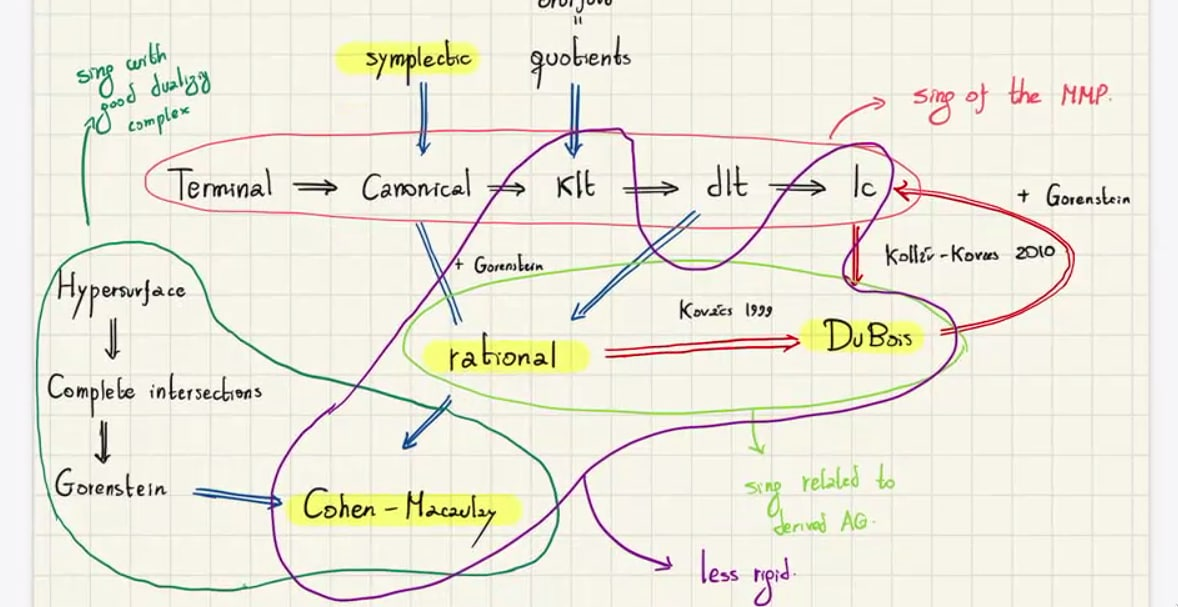
\includegraphics[width=0.8\linewidth]{sing}
    \caption{Map of singularities}%
    \label{fig:sing}
\end{figure}

We will now define some of these singularity classes and prove some of the implications.

\begin{defn}
    Let $(R, \mf{m})$ be a Noetherian local ring and $N$ be a finite $R$-module. Write $\dim N = \dim \supp N$. Then $N$ is called \textit{Cohen-Macaulay} of one of the following equivalent conditions holds:
    \begin{enumerate}
        \item There exists $x_1, \ldots, x_r \in \mf{m}$, where $r = \dim N$ such that $x_i$ is not a zero divisor in $N/(x_1, \ldots, x_{i-1})N$ for all $i$. Here, $x_1, \ldots, x_r$ is called a \textit{$N$-regular sequence}.
        \item If $x_1, \ldots, x_r \in \mf{m}$ for $r = \dim N$ and $\dim N/(x_1, \ldots, x_r)M = 0$, then $x_1, \ldots, x_r$ is an $N$-regular sequence.
    \end{enumerate}
    A coherent sheaf $\msc{F}$ on a scheme $X$ is \textit{Cohen-Macaulay} if $\msc{F}_x$ is Cohen-Macaulay over $\msc{O}_{X,x}$ for every $x \in X$. Finally, a scheme $X$ is \textit{Cohen-Macaulay} if its structure sheaf $\msc{O}_X$ is Cohen-Macaulay.
\end{defn}

There is a condition of Serre, which is slightly weaker than being Cohen-Macaulay. We say that a ring $R$ satisfies the properties
\begin{description}
    \item[$(R_k)$:] For all $\mf{p} \in \Spec A$ such that $\mr{ht}(\mf{p}) \leq k$, then $A_{\mf{p}}$ is regular.
    \item[$(S_k)$:] For all $\mf{p} \in \Spec A$, $\operatorname{depth}(A_{\mf{p}}) \geq \inf (k, \mr{ht}(\mf{p}))$.
\end{description}

\begin{exms}
    Normality is equivalent to $R_1$ and $S_2$, so all normal surfaces are Cohen-Macaulay. If $R$ is Cohen-Macaulay and a group $G$ acts on $R$, then $R^G$ is Cohen-Macaulay by Hochster-Roberts. This means that quotient singularities are Cohen-Macaulay. The rings $k[x]/x^2$ and $k[t^2, t^3]$ are Cohen-Macaulay. However, the scheme $X = \Spec k[x,y]/(x^2, xy)$ is \textbf{not} Cohen-Macaulay at the origin.
\end{exms}

\begin{defn}
    Let $Y$ be a variety over a field of characteristic $0$ and $X \xrightarrow{f} Y$ be a resolution of singularities. We say that $f$ is \textit{rational} if 
    \begin{enumerate}
        \item $f_* \msc{O}_X = \msc{O}_Y$ (here, $Y$ is normal).
        \item The higher derived pushforwards are given by $R^i f_* \msc{O}_X = 0$ for $i > 0$.
    \end{enumerate}
    We say that $Y$ has \textit{rational singularities} if every resolution is rational.
\end{defn}

Equivalently, the morphism $\msc{O}_Y \to R f_* \msc{O}_X$ is a quasi-isomorphism in the derived category.

\begin{exms}
    All singularities of the form $A_n$ are rational. If $X \to Y = A_n$, then $f^*(K_Y) = K_X$, so $Y$ is rational. However, the cone over an elliptic curve is not rational.
\end{exms}

\begin{defn}
    A point $y \in Y$ is \textit{symplectic} if $Y$ is normal at $y$ and there exists a symplectic form $\omega$ on $Y^{\mr{reg}}$ which extends to the exceptional divisor over $y$ on any resolution.
\end{defn}

\begin{defn}
    Let $X \subseteq Y$ be an embedding of a scheme into a regular scheme and $Z \to Y$ be a log resolution of $X$ which is an isomorphism outside $X$. Let $E$ be the reduced preimage of $X$ in $Z$. Then we say $X$ has \textit{Du Bois singularities} if $\msc{O}_X \to R\pi_* \msc{O}_E$ is a quasi-isomorphism.
\end{defn}

\begin{rmk}
    Du Bois singularities commonly appear in Hodge theory.
\end{rmk}

\begin{rmks}\leavevmode
    \begin{itemize}
        \item Serre duality for Cohen-Macaulay sheaves
        \item If $H \subseteq X$ is Cartier and $H$ is Cohen-Macaulay, then so is $X$.
    \end{itemize}
\end{rmks}

\begin{prop}
    Let $Y$ be a variety over a field of characteristic $0$ and $f \colon X \to Y$ be a resolution. The following are equivalent:
    \begin{enumerate}
        \item $f$ is rational.
        \item $Y$ is Cohen-Macaulay and $f_* \omega_X = \omega_Y$.
    \end{enumerate}
\end{prop}

\begin{proof}
    Let $Y$ be projective and $D$ be an ample Cartier divisor on $Y$. Then $H^i(X, \omega_X(rf^* D)) = 0$ for $r > 0, r > 0$. By Serre duality, we have $H^{n-i}(X, \msc{O}_X(-rf^* D)) = 0$ for $i > 0$ and $r > 0$. Then the Leray spectral sequence
    \[ E_2^{i,j} = H^i(Y, R^j f_* \msc{O}_X(-rD)) \Rightarrow H^{i+j}(X, \msc{O}_X(-rf^* D)). \]
    Assuming that $f$ is rational, we then obtain
    \[ H^i(Y, \msc{O}_Y(-rD)) \simeq H^i(X, \msc{O}_X(-rf^* D)) \qquad i > 0. \]
    Now we will prove that $H^i(Y, \msc{O}_Y(-rD)) = 0$ for $i < n$ and $r \gg 0$ only if $Y$ is Cohen-Macaulay.\footnote{The other direction is true, but we do not need it right now.} Let $H \subseteq \abs{r'D}$ be a general element. We obtain the exact sequence
    \[ 0 \to \msc{O}_Y(-(r+r')D) \xrightarrow{\cdot H} \msc{O}_Y(-rD) \to \msc{O}_H(=rD) \to 0. \]
    By vanishing, we see that $H^i(H, \msc{O}_H(-rD))$ for $i < n-1$ and $r \gg 0$. Therefore by induction, $H$ is Cohen-Macaulay and thus $Y$ is Cohen-Macaulay. Taking the case of $i = 0$, we obtain
    \[ h^0(Y, \omega_Y(rD)) = h^0(X, \omega_X(rf^*D)) = h^0(Y, f_* \omega_X(rD)) \]
    for all $r > 0$. This implies that $f_* \omega_X = \omega_Y$ by a result in Hartshorne.

    Now assume that $Y$ is Cohen-Macaulay and $f_* \omega_X = \omega_Y$. We will induct on the dimension, and CM curves are smooth, so we proceed to the inductive step. We will prove that $R^i f_* \msc{O}_X$ is supported in some $0$-dimensional locus. Let $H \subseteq Y$ be general and $H' = f^{-1}H$, so $f \colon H' \to H$ is a resolution. Then 
    \[ f_* \omega_{H'} = f_* (\omega_X(H') \otimes \msc{O}_{H'}) = \msc{O}_H(H) \otimes f_* \omega_X = \msc{O}_H(H) \otimes \omega_Y = \omega_H. \]
    By induction, we see that $\msc{O}_H \otimes R^i f_* \msc{O}_X = R^i f_* \msc{O}_{H'} = 0$ is trivial outside a zero dimensional set. Therefore $H^0(Y, R^q f_* \msc{O}_X(-rD)) = 0$ for $p,q > 0$ or if $p<n$ and $q=0$. By the spectral sequence, we obtain $H^0(Y, R^q f_* \msc{O}_X \otimes_{\msc{O}_Y} \msc{O}_Y(-rD)) = 0$ for $q < n-1$ and
    \[ H^0(Y, R^{n-1}f_* \msc{O}_X(-rD)) \cong \ker \qty[ H^n(Y, \msc{O}_Y(-rD)) \xrightarrow{\alpha} H^n(X, \msc{O}_X(-rf^* D)) ]. \]
    This implies that $R^q f_* \msc{O}_X = 0$ for $q < n-1$. When $q = n$, $\alpha$ is the dual to the morphism
    \[ H^0(Y, \omega_Y(rD)) \to H^0(X, \omega_X(rf^*D)) = H^0(Y, f_* \omega_X(rD)) \]
    because $\omega_Y \simeq f_* \omega_X$. Thus $\alpha$ is an isomorphism and thus $R^n f_* \msc{O}_X = 0$.
\end{proof}

\begin{lem}
    Let $(X, \Delta)$ be a klt pair, $H$ be basepoint free, and $H_g \in \abs{H}$ be a general element. Then $(H, \delta_H)$ is klt.
\end{lem}

\begin{lem}
    Let $Y \xrightarrow{f} X$ be finite with $K_Y + \Delta_Y = f^*(K_X + \Delta)$. Then if both $(X, \Delta), (Y, \Delta_Y)$ are log pairs, then $(X, \Delta)$ is klt (resp.~log canonical) if and only if $(Y, \Delta_Y)$ is klt (resp.~log canonical).
\end{lem}

The idea of the proof is to use the Riemann-Hurwitz formula on a log resolution to compare the discrepancies and observe that $a_E(X, \Delta) = ra_E(Y, \Delta_Y)$ for some positive integer $r$ (a ramification index).

\begin{thm}[Elkik 1981]
    If $(X, \Delta)$ is dlt, then $X$ has rational singularities.
\end{thm}

\begin{proof}
    Write $K_Y \equiv f^*(K_X + \Delta) + A - B$, where $Y \to X$ is a log resolution, $\Supp B \subseteq \operatorname{Ex}(f)$, and $\floor{A} = 0$. By KV vanishing, $R^j f_* \msc{O}_Y(\ceil{B}) = 0$ for $j > 0$. Now let $\msc{L}$ be an ample Cartier divisor on $X$. WE have a commutative diagram
    \begin{equation*}
    \begin{tikzcd}
        H^i(\msc{O}_Y(-rf^* \msc{L})) \ar{r} & H^i(\msc{O}_Y(\ceil{B} - rf^* \msc{L})) \\
        H^i(\msc{O}_X(-r\msc{L})) \ar{u} \ar[equal]{r} & H^i(\msc{O}_X(-r\msc{L})). \ar{u}{\beta}
    \end{tikzcd}
    \end{equation*}
    Therefore we have
    \[ H^i(X, \msc{O}_X(-r\msc{L}) \otimes R^j f_* \msc{O}_X(\ceil{B})) \Rrightarrow H^{i+j}(Y, \msc{O}_Y(\ceil{B} - rf^*\msc{L})) \]
    and $H^i(\msc{O}_Y(-rf^* \msc{L})) = 0$ for $i < n$ and $r > 0$ by KV vanishing. We want to conclude that $H^i(\msc{O}_X(-r\msc{L})) = 0$ for $r > 0, i < n$. Using vanishing and the spectral sequence, we see that $\beta$ is an isomorphism. But then by vanishing again, the top left corner is $0$, and thus everything in the diagram must vanish. Therefore $X$ is Cohen-Macaulay.

    Now if we take $j = 0$, we obtain an injection $H^n(\msc{O}_X(-r\msc{L})) \hookrightarrow H^n(\msc{O}_Y(-rf^*\msc{L}))$. By Serre duality, the map $H^0(Y, \omega_Y(rf^*\msc{L})) = H^0(X, f_*\omega_Y \otimes \msc{O}_X(r\msc{L})) \twoheadrightarrow H^0(X, \omega_X \otimes \msc{O}_X(r\msc{L}))$ is a surjection, and surjectivity for $r \gg 0$ implies that $f_* \omega_Y \twoheadrightarrow \omega_X$, and they are isomorphic because they are both rank $1$ reflexive sheaves. Therefore $X$ has rational singularities.
\end{proof}

\begin{prop}
    If $X$ is Gorenstein (this means $K_X$ is Cartier), then rational is equivalent to canonical.
\end{prop}

\begin{proof}
    We know canonical implies dlt implies rational. Now suppose that $X$ is rational and Gorenstein and let $Y \xrightarrow{\pi} X$ be a resolution. Then $\pi^*(K_X) = K_Y + E - F$, where $E, F$ are integral and effective with no common support. To prove that $X$ is canonical, we need to prove that $E = 0$. If we push-forward $K_Y + E - F$ and $E \neq 0$, then we get associated primes on the image of $E$, and this contradicts $\pi_* \omega_Y = \omega_X$. Therefore $E$ is trivial, so $X$ is canonical.
\end{proof}

\begin{prop}
    Symplectic singularities are rational and Gorenstein.
\end{prop}

\begin{proof}
    Let $\pi \colon Y \to X$ be a resolution. If $\varphi$ be a $2$-form, then $\varphi^r$ generates the line bundle $\omega_{X^{\mr{reg}}}$. The fact that $\pi^* \varphi$ extends to a regular holomorphic form implies that $\pi^* \varphi^r$ extends. Thus $\pi_* \omega_Y = \pi_* (\pi^*\varphi^r) = \varphi^r = \omega_X$. In addition, we see that $\pi^*\omega_X = \omega_Y - F$.
\end{proof}

We can characterize the condition of being Gorenstein as follows: A local ring $(R, \mf{m})$ is Gorenstein if and only if there exists a regular sequence $x_1, \ldots, x_r$ such that $R/(x_1, \ldots, x_r)$ is Gorenstein and $0$-dimensional. By Nakayama's lemma, this implies that $R/(x_1, \ldots, x_i) R$ is Gorenstein for every $i$.

\begin{lem}
    Let $(0 \in X)$ be an index $1$ canonical threefold singularity and $0 \in H \subseteq X$ be a general hyperplane section. Then either $(0 \in H)$ is a Du Val singularity or an elliptic singularity.
\end{lem}

The idea of the proof is that if $H' \xrightarrow{\pi} H$ is a resolution, then $\pi_* \omega_{H'} = m \omega_H$. If $m = 1$, we have a Du Val singularity, and if $m > 1$, then we have an elliptic singularity.

\begin{thm}
    All terminal threefold singularities of index $1$ are cDV (compound Du Val), which means a one-parameter deformation of a Du Val singularity.
\end{thm}

\begin{exm}
    Let $G \subseteq GL_n(\C)$ be a finite group. We know $\C^n/G$ is a quotient singularity and thus klt. If $G \subseteq SL_n(\C)$, then $\C^n/G$ is symplectic.
\end{exm}

\begin{exm}
    If $x \in X$ is a cone and is symplectic, then it is isomorphic to a Lie group quotient by the smallest nonzero nilpotent orbit.
\end{exm}

\section{Duality Theory}%
\label{sec:duality_theory}

Given a projective variety $X$, we want a sheaf $\omega_X$ such that $H^i(X, \msc{F}) = { H^{n-i}(X, \msc{H}om(\msc{F}, \omega_X)) }^{\vee}$ for every Cohen-Macaulay sheaf. Recall that Serre duality establishes this duality for $H^n(\P^n, \msc{F}) = \Hom(\msc{F}, K_{\P^n})$ for any quasicoherent sheaf. Moreover, if $\msc{F}$ is locally free, then
\[ H^i(\P^n, \msc{F}) = { H^{n-i}(\P^n, K_{\P^n} \otimes \msc{F}^*) }^{\vee}. \]
\begin{defn}
    A \textit{dualizing sheaf} $\omega_X$ is a coherent sheaf with a surjection
    \[ \Tr_X \colon H^n(X, \omega_X) \to k \]
    such that for all coherent $\msc{F}$, $\Tr_X$ induces an isomorphism
    \[ \Hom (\msc{F}, \omega_X) = \Hom(H^n(X, \msc{F}, k)). \]
    The pair $\omega_X, \Tr_X$ is unique if it exists.
\end{defn}

\begin{prop}
    Let $f \colon X \to Y$ be a finite morphism, $\msc{F} \in \mr{Coh}(X), \msc{G} \in \mr{Coh}(Y)$. Let $f^! \msc{G} \coloneqq \msc{H}om_{\msc{O}_Y}(f_* \msc{O}_X, \msc{G})$,
    \begin{enumerate}
        \item There exists an isomorphism $f_* \msc{H}om(\msc{F}, f^! \msc{G}) = \msc{H}om_{\msc{O}_Y}(f_* \msc{F}, \msc{G})$.
        In particular, there is a natural isomorphism $\Hom_X(\msc{F}, f^! \msc{G}) = \Hom_Y(f_* \msc{F}, \msc{G})$.
    \end{enumerate}
\end{prop}

\begin{proof}
    Assume $X = \Spec A, Y = \Spec B$ and $\msc{F} = \wt{M}, \msc{G} = \wt{N}$. Then we have reduced to the identity
    \[ \Hom_A(M, \Hom_B(A, N)) = \Hom_B(M, N), \]
    but this is obvious. Simply write $\psi(m)(a) = \phi(am)$ for some $\phi \in \Hom_B(M, N)$.
\end{proof}

\begin{proof}
    Let $f \colon X \to Y$ be a finite morphism of proper schemes of pure dimension $m$. If $\omega_Y$ exists, then $\omega_X$ exists and $\omega_X = f^! \omega_Y$.
\end{proof}

\begin{proof}
    We simply compute
    \begin{align*}
        \Hom_X(\msc{F}, \omega_X) &= \Hom_X(\msc{F}, f^! \omega_Y) \\
                                  &= \Hom_Y(f_* \msc{F}, \omega_Y) \\
                                  &= { H^m(Y, f_* \msc{F}) }^{\vee} \\
                                  &= { H^n(X, \msc{F}) }^{\vee}.
    \end{align*}
    Here, finiteness gives us $R^i f_* \msc{F} = 0$ for $i > 0$ and thus the Leray spectral sequence applies.
\end{proof}

\begin{cor}
    The sheaf $\omega_X$ exists and is an $S_2$-sheaf for projective varieties $X$ over $k$.
\end{cor}

\begin{proof}
    We always have a finite surjective morphism $X \to \P^n$ (embed in large projective space, then project down). Then $\omega_{\P^n}$ exists, so $\omega_X$ does also. Also $\omega_X$ is $S_2$ if and only if $f_* \omega_X$ is, but $f_* \omega_X = \msc{H}om(\text{locally free})$. 
\end{proof}

\begin{cor}
    If $X$ is a projective scheme of pure dimension $m$ over $k$, $\msc{F}$ a coherent sheaf such that $\supp \msc{F}$ has pure dimension $m$, then
    \begin{enumerate}
        \item If $\msc{F}$ is Cohen-Macaulat, so is $\msc{H}om(\msc{F}, \omega_X)$. The converse holds if $\msc{F}$ is $S_2$.
        \item If $X$ is $S_2$, then $\msc{O}_X$ is Cohen-Macaulay if and only if $\omega_X$ is.
    \end{enumerate}
\end{cor}

\begin{proof}
    Let $f \colon X \to \P^m$ be surjective and finite. Then $\msc{F}$ is Cohen-Macaulay if and only if $f_* \msc{F}$ is locally free, so $\msc{H}om_{\msc{O}_X}(\msc{F}, \omega_X)$ is Cohen-Macaulay if and only if
    \[ f_* \msc{H}om_{\msc{O}_X} (\msc{F}, \omega_X) = \msc{H}om_{\msc{O}_{\P^n}}(f_* \msc{F}, \omega_{\P^n}), \]
    and $f_* \msc{F}$ is locally free if and only if $\msc{F}$ is $S_2$.
\end{proof}

\begin{thm}
    Let $X$ be a projective scheme of pure dimension $m$, $\msc{F}$ a Cohen-Macaulay sheaf such that $\supp \msc{F}$ has pure dimension. Then
    \[ H^i(X, \msc{F}) = {H^{n-i}(X, \msc{H}om_{\msc{O}_X}(\msc{F}, \omega_X))}^{\vee}. \]
\end{thm}

\begin{proof}
    As before, let $f \colon X \to \P^m$ be finite and surjective. We know that $H^i(X, \msc{F}) = H^i(\P^m, f_* \msc{F})$. Then $f_* \msc{F}$ is locally free, so by Serre duality, we have
    \[ H^i(\P^m, f_* \msc{F}) = { H^{m-i}(\P^m, \msc{H}om_{\msc{O}_{\P^m}}(f_* \msc{F}, \omega_{\P^m})) }^{\vee}, \]
    and therefore we obtain
    \[ H^{m-i}(\P^m, \msc{H}om(f_* \msc{F}, \omega_{\P^m})) = H^{m-i}(\P^m, f_* \msc{H}om_{\msc{O}_X}(\msc{F}, \omega_X)) = H^{m-i}(X, \msc{H}om_{\msc{O}_X}(\msc{F}, \omega_X)). \qedhere \] 
\end{proof}

\begin{prop}
    Let $X$ be a projective Cohen-Macaulay scheme of pure dimension $m$, $D \subset X$ a Cartier divisor. Then $\omega_D = \omega_X(D) \otimes \msc{O}_D$. 
\end{prop}

\begin{prop}
    Let $X$ be a normal projective variety of dimension $m$. Then $\omega_X = \msc{O}_X(K_X)$.
\end{prop}

These two facts tive the classical \textit{adjunction formula}.
\begin{prop}
    Let $X$ be smooth and $D \subset X$ be a smooth Cartier divisor. Then $\eval{(K_X + D)}_D = K_D$.
\end{prop}

Next, we want to compare singularities of $(X, B+S)$ with $\qty(S, \eval{B}_S)$. 

\begin{rmk}
    If $S$ is Cartier in codimension $2$, then $\eval{(K_X + B + S)}_S = K_S + \eval{B}_S$. If there are quotient singularities in codimension $2$, then $\eval{(K_X + B + S)}_S = K_S + \eval{B}_S + \sum_{P_i} \qty(1 - \frac{1}{m_i}) P_i$, where $P_i$ is a codimension $2$ point of $X$, orbifold of order $m_i$.
\end{rmk}

The idea of adjunction is that if $(X, B+S)$ has nice singularities, then so does $\qty(S, \eval{B}_S)$. The convsers is called the inverse of adjunction.

\begin{prop}
    Let $X$ be normal and $S$ be a normal Weil divisor that is Cartier in codimension $2$.  Let $Z \subseteq X$ be closed and $B = \sum b_i B_i \geq 0$. Assume that $K_X + S + B$ is $\Q$-Cartier. Then
    \[ \text{tot.disc}\qty(\text{center} \subseteq Z, S, \eval{B}_S) \geq \text{discrep}(\text{center} \subseteq Z, X, S+B) \geq \text{discrep}(\text{center} \cap S \subseteq Z, X, S + B). \]
\end{prop}

\begin{proof}
    Let $f \colon Y \to X$ be a log-resolution of $(X, S+B)$ and write $S' = f_*^{-1} S$ and $f_*^{-1}(S + B)$ is smooth. By doing more blowups, we may assume that if $E_i$ ie exceptional such that $E_i \cap S' \neq \emptyset$, then the center of $E_i$ is contained in $S$. We have
    \[ K_Y + S' \equiv f^*(K_X + S + B) + \sum e_i E_i \] and $K_{S'} = \eval{(K_Y + S')}_{S'}$, and therefore
    \[ K_{S'} \equiv f^* \qty( \eval{(K_S + B)}_S ) + \sum e_i (E_i \cap S'). \]
    Now $S'$ is distinct from $f_*^{-1}B$, so if $E_i \cap S' \neq \emptyset$, then $E_i$ is $f$-exceptional and the center of $E_i$ is contained in $S$. this shows that every log discrepancy that happens in $S' \to S$ also happens in $Y \to X$ in such a way that the center lies inside $S$.
\end{proof}

Therefore, if $(X, B+S)$ is plt, then $\qty(S, \eval{B}_S)$ is klt. The inverse of adjunction is more difficult. Suppose that $\qty(S, \eval{B}_S)$ has nice singularities, but $(X, B+S)$ has bad singularities. In particular, there exist exceptional $E$ over $X$ such that $a_E(X, B+S) < 0$. This contradicts the philosophy that in a Fano object, the locus where it's more singular is contracted. The theorem that realizes this is called \textit{Koll\`ar-Shokurov connectedness}.

\begin{defn}
    Let $(X, B)$ be a log-canonical. We say that $Z \subseteq X$ is a \textit{log-canonical center} if there exists $E$ over $X$ with $a_E(X, B) = 0$ and $c_E(X) = Z$. We denote by $lcc(X, B)$ the union of all log-canonical centers. This is a closed subset.
\end{defn}

\begin{thm}[Kolla\`ar-Shokurov connectedness]
    Let $f \colon X \to Z$ be projective, $(X, B)$ be log-canonical, and $-(K_X + B)$ be ample over $Z$. Then $lcc(X, B)$ is connected over $Z$.
\end{thm}

\begin{exm}
    Let $\P^1 \to \mr{pt}$ be the structure morphism and note that $\deg K_{\P^1} = -2$. The coefficients of the dropped points must have sum stricly less than $2$.
\end{exm}

\begin{rmk}
    Big and nef suffices in place of ample.
\end{rmk}

\begin{thm}
    Let $g \colon Y \to X$ be a proper birational mapping with $Y$ smooth and $X$ normal. Let $D = \sum d_i D_i$ be a smooth normal crossings $\Q$-divisor on $Y$ such that $g_* D \geq 0$ and $-(K_Y + D)$ is $g$-nef. Write
    \[ A = \sum_{i, d_i < 1} d_i D_i, \qquad F = \sum_{i, d_i \geq 1} d_i D_i. \]
    Then $\supp F = \supp \floor{F}$ is connected in any neighborhood of any fiber of $g$.
\end{thm}

\begin{rmk}
    A field $K$ is $C_1$ if every homogeneous $f(x_0, \ldots, x_n) \in K[x_0, \ldots, x_n]$ of degree at most $n$ has a nontrivial zero. A field is \textit{pseudo-algebraically closed} if every geometrically integral $k$-variety has a $k$-point.
\end{rmk}

\begin{conj}[Ax]
    Every pseudo-algebraically closed field of characteristic $0$ is $C_1$.
\end{conj}

This is true and proved by Koll\`ar.

\begin{proof}[Proof of Theorem]
    Note that $\ceil{-A} - \floor{F} = K_Y - g^*(K_X + D) + \qty{A} + \qty{F}$. By KV vanishing, we have $R^1 g_* \msc{O}_Y(\ceil{-A} - \floor{F}) = 0$. Then we have the exact sequence
    \[ 0 \to \msc{O}_Y(\ceil{-A} - \floor{F}) \to \msc{O}_Y(\ceil{-A}) \to \msc{O}_{\floor{F}}(\ceil{-A}) \to 0 \]
    so $g_* \msc{ O }_Y(\ceil{-A}) \twoheadrightarrow g_* \msc{O}_{\floor{F}}(\ceil{-A})$. Now $\ceil{-A}$ is $g$-exceptional, so $g_* \msc{O}_Y(\ceil{-A}) = \msc{O}_X g_* D \geq 0$. Writing $\floor{F} = F_1 \cup F_2$ is a neighborhood of $h^{-1}(x)$, we obtain
    \[ { g_* \msc{O}_{\floor{F}}(\ceil{-A}) }_{(x)} = { g_* \msc{O}_{F_1} (\ceil{-A}) }_(x) + g_* \msc{O}_{F_2}(\ceil{-A}). \]
    This will give a surjection $\msc{O}_{X, x} \to \msc{O}_{\floor{F}, x}$, which is not true by connectedness.
\end{proof}

\begin{thm}
    Let $X$ be normal and $S \subseteq X$ be a normal Weil divisor Cartier in codimension $2$. Let $B \geq 0$ be a $\Q$-divisor such that $K_X + S + B$ is $\Q$-Cartier. Then
    \begin{enumerate}
        \item $(X, S+B)$ is plt near $S$ if and only if $\qty(S, \eval{B}_S)$ is klt.
        \item Assume $B$ is $\Q$-Cartier and $S$ it klt. Then $(X, S+B)$ is log canonical near $S$ if and only if $\qty(S, \eval{B}_S)$ is log canonical.
    \end{enumerate}
\end{thm}

\begin{proof}
    Take $g \colon Y \to X$ a log resolution of $(X, S+B)$ and $K_Y + D = g^*(K_X+B+S)$. Write $S' = g_*^{-1} S$ and $F = S' + F'$. Then $F'$ contains a component of codimensino at least $1$. By adjunction, we have 
    \[ K_{S'} = g_* \qty(K_X + \eval{B}_S) + \eval{(A-F')}_{S}, \]
    so $(K, B+S)$ is plt near $S$ if and only if $F' \cap g^{-1}(S) = \emptyset$ and $\qty(S, \eval{B}_S)$ is klt if and only if ${(F')}^{\geq 0} \cap S' = \emptyset$. By Koll\`ar-Shokurov connectedness, given $x \in S$, there exists $V_x \subseteq X$ such that $(S' \cup {(F')}^{\geq 1}) \cap g^{-1}(V_x)$ is connected. Here $F' \cap g^{-1}(V_x) = \emptyset$. Moving $x$ around $S$ finishes the argument. 
\end{proof}

We will now consider adjunction for higher codimension centers. We know $(X, S+B)$ is snc if and only if $\qty(X, \eval{B}_S)$ is. For $(X, B)$, let $Z$ be a log-canonical center on $(X, B)$. If $Z$ has codimension $1$ in $X$, do adjunction to $Z$ and repeat. If $Z$ has codimension at least $2$, define $(Z, B_Z)$ such that the singularities of $(X, B)$ around $Z$ can be compared to those of $(Z, B_Z)$.

This is indeed possible. First blow up enough so that $g$ maps $E$ to $Z$. Write $g^*(K_X + B) = K_Y + B_Y + E$. Then we have
\[ \eval{g^*(K_X + B)}_E = \eval{ ( K_Y + B_Y + E ) }_E = K_E + B_E \]
and this is trivial over $Z$. We want to write $K_E + B_E = g^*(K_Z + B_Z + M_Z)$, where $B_Z$ measures the singularities of the fiber $M_Z$, the variation of moduli.

\section{Terminal threefold MMP}%
\label{sec:terminal_threefold_mmp}

Let $X$ be a $\Q$-factorial terminal projective threefold and $X \xrightarrow{f} W$ be a flipping contraction. Suppose $\rho(X/W) = 1$, $-K_X$ is ample over $W$, and $X$ has terminal singularities and is smooth in codimension $2$. First, we want to construct a rational map $\pi$ which is an isomorphism in codimension $1$ such that $\rho(X^+/W) = 1$, $K_{X^+}$ is ample over $W$, and $X^+$ has terminal singularities. Also, $X^+$ is unique and coincides with
\[ \Proj_W \bigoplus_{n \geq 0} f_* \msc{O}_X(nK_X) \]
provided that this ring is a finitely generated $\msc{O}_W$-algebra. Denote this ring by $R(X)$.

\begin{prop}
    The ring $R(X)$ is finitely generated as an $\msc{O}_W$-algebra if and only if it is finitely generated locally over $W$ (and this is even true locally analytically).
\end{prop}

For a geometric picture, let $X$ be a terminal threefold and suppose $f$ contracts several curves. Then $W$ is not $\Q$-factorial in general. In 1988, Mori proved that these curves can be contracted one-by-one \textbf{in the analytic category} (in the algebraic category, this is clearly impossible by the previous discussion). Now our terminal threefold flipping contractions lead us to studying extremal neighborhoods. Here, we consider an analytic neighborhood of the fiber above $w \in W$. We may assume that $(W, w)$ is a rational singularity. Now what happens if our extremal neighborhood is smooth?

\begin{prop}
    Let $X \supseteq C = \P^1$ be an extremal neighborhood. Then $\msc{O}_C(K_X) = \msc{O}_C(-1)$, $\msc{I}_C / \msc{I}_C^2 \simeq \msc{O}_C \oplus \msc{O}_C(1)$, and $\abs{-K_X}$ has a smooth member.
\end{prop}

\begin{proof}
    We know that $K_X. C = -1$ because $K_X. C < 0$ and $H^1(\msc{O}_C(K_X)) = 0$. Now we have an exact sequence
    \[ 0 \to \msc{I}_C/\msc{I}_C^2 \to \Omega^1_X \otimes \msc{O}_C \to \msc{O}(K_C) \to 0, \]
    and thus we have an isomorphism $\bigwedge^2(\msc{I}_C/\msc{I}_C^2) \simeq \msc{O}(K_X) \otimes \msc{O}_C(-K)$. Taking the degree, we conclude that $\deg \msc{I}_C / \msc{I}_C^2 = (-K_X.C) - \deg K_C = 1$. Now if we tensor with $\msc{O}_C(-1)$, we obtain the exact sequence
    \[ 0 \to \msc{I}_C/\msc{I}_C^2 \otimes \msc{O}_C(-1) \to \msc{O}_X / \msc{I}_C^2 \otimes \msc{O}_X(K_X) \to \msc{O}_C(-1) \to 0. \]
    Because $H^1(\msc{I}_C / \msc{I}_C^2 \otimes \msc{O}_C(-1)) = 0$, we have $\msc{I}_C / \msc{I}_C^2 \otimes \msc{O}_C(-1) \simeq \msc{O}_C(-1) \oplus \msc{O}_C$.

    Now let $x \in C$ and $(D, x)$ be a smooth divisor on the germ $(X, x)$. Then $D$ extends naturally to a divisor $D'$ of $X$. We need to show that $D' \in \abs{-K_X}$. Here, we know that $\Pic X = \Z$ and the isomorphism is induced by $\msc{L} \mapsto \msc{L}.C$. Thus $D' \sim -K_X$.
\end{proof}

\begin{cor}
    In the above case, $X$ is the blowup of a smooth threefold $(W, w)$ along a smooth curve $C_0 \ni w$.
\end{cor}

\begin{cor}
    Let $X \to W$ be a terminal threefold flipping contraction. For every $w \in W$, $f^{-1}(W)$ contains a singularity.
\end{cor}

By the classification of terminal threefold singularities, for any extremal neighborhood, there are at most three singular points and there is a nice divisor $D$ passing through some of them.

\begin{thm}[Mori 1988]
    Let $X \supseteq C = \P^1$ be an extremal neighborhood. Then one of the following holds for $\abs{-aK_X}$ ($a = 1, 2$):
    \begin{enumerate}
        \item Either $\abs{-K_X}$ has a member $D$ with Du Val singularities, or
        \item $\abs{-2K_X}$ has a member $D$ such that the double cover $Z$ of $X$ branched over $X$ with only Du Val singularities.
    \end{enumerate}
\end{thm}

Because $D$ is Du Val, we know $(X, D)$ is purely log terminal. Now the finite generation of the ring $R(X)$ is implied by the finite generation of the ring
\[ \bigoplus_{n \geq 0} \eval{f}_D \msc{O}_D(nK_X). \]
This is now a problem about projective surfaces, and apparently this is doable by hand. Here, $D$ is a log-Calabi Yau surface with at most three singular points. Now we conclude the existence of flips for terminal threefolds.

Now we need to prove termination of flips. 

\begin{thm}
    An arbitrary sequence of three-dimensional extremal canonical $(K_X + \Delta)$-flips is finite.
\end{thm}

\begin{lem}
    Let $\phi \colon X \dashrightarrow X'$ be a $(K_X + \Delta)$-flip of a three=dimensional canonical pair $(X, \Delta)$, where $\Delta = \sum a_i D_i$. Let $C' \subseteq X'$ be a flipped curve and $E_{C'}$ be the exceptional divisor obtained by blowing up $C'$. Then $X'$ is smooth along $C'$ and 
    \[ 0 \leq a(E_{C'}, X, \Delta) < a(E_{C'}, X', \Delta') = 1 - \sum a_i \text{mult}_{C'} (D_i'), \]
    where the multiplicities are of $D'$ along $C'$.
\end{lem}

\begin{proof}
    Because $C'$ is a flipped curve, $X'$ is smooth along the generic point of $C'$. Indeed, $X'$ is terminal along $\eta_{C'}$, so it is smooth. If there is a nonterminal valuation with center on $C'$, then there is a noncanonical valuation on $(X, \Delta)$.
\end{proof}

We will now define the \textit{difficulty function}. Let $\qty(X, \Delta = \sum a_i D_i)$ be a canonical pair with $D_i$ pairwise distinct prime divisors. Set $a = \max \qty{a_i}$ and $S \coloneqq \sum a_i \Z_{\geq 0} \subseteq \Q$. Also write
\[ d(X, \Delta) = \sum_{\substack{x \in S \\ x \geq a}} \# \qty{\text{Exceptional divisors over $X$ with $a(E, X, \Delta) < 1-x$}}. \]
For example, with compound Du Val singularities, we have $d(cDv) = r$.

\begin{rmk}
    The difficulty function measures the number of nonterminal valuations.
\end{rmk}

We are now ready to prove termination of canonical threefold flips.

\begin{proof}[Proof of termination of flips]
    Write $\Delta = \sum a_i D_i$, where $a_1 \leq \cdots \leq a_k$. Then in the sequence of flips, we have 
    \[ (X, \Delta) \dashrightarrow (X^1, \Delta^1) \dashrightarrow (X^2, \Delta^2) \dashrightarrow \cdots \]
    If $k = 0$, then $d(X^{k-1}, 0) > d(X^j, 0)$. Therefore, after finitely many flips, $d(X^{\ell}, 0) = 0$ and thus there are no more flips.

    Now assume that $k > 0$. Then we know $d(X^j, \Delta^j)$ is nondecreasing. If $C^j$ is the flipped curve for $\phi^{j-1}$, assume it is contained in $D_k^j$. Then $a_k < 1$ and $d(X^{j-1}, \Delta^{j-1}) > d(X^j, \Delta^j)$. Therefore for $j \gg 0$, $D_k^j$ contains no flipped curves.

    Now denote by $\ol{D}_k^j$ the normalization of $D_k^j$. Then $\ol{D}_k^{j-1} \to \ol{D}_k^j$ is a birational morphism. The exceptional curves of $\ol{D}_k^j \to \ol{D}_k^{\ell}$ for $\ell > k$ are linearly independent. At some point, we have $\ol{D}_k^j \simeq \ol{D}_k^{\ell}$ for $\ell \gg j$. This means that both the flipping and flipped curves are disjoint from $D_k^j$. Thus $C.D_k^j = 0$, so now flips for $\qty(X, \Delta = \sum_{i=1}^k a_i D_i)$ induce flips on $\qty(X, \Delta' = \sum_{i=1}^{k-1} a_i D_k)$, and by induction, these flips stop.
\end{proof}

\begin{conj}[Abundance]
    If $X$ is klt and $K_X$ is nef, then $K_X$ is semiample.
\end{conj}

This is proved for terminal threefolds by Kawamata. Now we have settled the minimal model program for terminal threefolds. Existence and termination of flips were proved in 1988 by Mori and later in a more general case by Koll\'ar-Shokurov, and abundance was proved by Kawamata in the 1990s. A historical sketch of more recent developments is as follows:

\begin{table}[H]
    \centering
    \caption{Historical Sketch since 2000}
    \label{tab:label}
    \begin{tabular}{p{0.45\textwidth}p{0.45\textwidth}}
    \toprule
    Existence of Flips & Termination of Flips \\
    \midrule
    In the 2000s Koll\'ar-Shokurov proved existence for $(X, \Delta)$ log-canonical threefolds & In 2004, Alexeev-Hacon-Kawamata proved termination for $(X, \Delta)$ fourfolds with $-(K_X + \Delta)$ effective. \\
    In 2005, Hacon and McKernan proved flips exist in dimension $n$ provided the MMP works in dimension $n-1$. & In 2000, Fujino proved termination of flips for $(X, \Delta)$ a terminal fourfold. \\
    In 2006, Birkar-Cascini-Hacon-McKernan proved existence of flips for $(X, \Delta)$ klt. & They also proved termination of flips for $(X, \Delta)$ klt and $K_X + \Delta$ big. \\
    In 2010, Hacon-Xu and Birkar proved exietence of flips for $(X, \Delta)$ log canonical. & In 2018, Joaqu\'{\i}n proved termination of flips for $(X, \Delta)$ a log canonical fourfold with $K_X + \Delta$ pseudoeffective. \\
    \bottomrule
    \end{tabular}
\end{table}

Termination is unknown for klt uniruled fourfolds and in dimension at least $5$. Abundance is known for log canonical pairs in dimension $3$ and log canonical pairs in dimension $4$ with $X$ uniruled. It is unknown for log canonical pairs with $K_X + \Delta$ pseudoeffective. Some people believe that abundance should be tackled using different techniques from the minimal model program.

\section{Applications to Singularities}%
\label{sec:applications_to_singularities}

Conjecturally, the MMP contracts or flips the locus $\mr{Bs}(K_X) = \mr{Bs}_-(K_X)$. This is known in dimension $3$ and follows from termination and abundance. Recall that if $D \subseteq X$ and $A$ is an ample divisor on $X$, then 
\[ \mr{Bs}-(D) = \bigcup_{\ep > 0} \mr{Bs}(D + \ep A) \subseteq \mr{Bs}(D). \]
This is a countable union of algebraic varieties. Then (someone) showed the existence of a divisor on a certain blowup of $\P^3$ whose $\mr{Bs}_-$ is a countable union of curves. Here, the dynamics of what happens lead to something non-algebraic.

The first application we will give is \textit{terminalization}. Let $(X, \Delta)$ be a klt pair. Then there exists a projective birational morphism $Y \to X$ such that $Y$ is terminal and extracts exactly the divisors with $a_E(X, \Delta) \in (-1,0]$.

To prove this, let $(Z, \Delta_Z) \xrightarrow{\varphi} (X, \Delta)$ be a log resolution of $X$. Then we know $\varphi^*(K_X + \Delta) = K_Z + \Delta_Z$. This is not necessarily a boundary, so write $\Delta_Z'$ for the result of killing all negative coefficients. By negativity, we see that $\mr{Bs}_-(K_Z + \Delta_Z')$ contains all divisors with $a_E(X, \Delta) > 0$. Now we run the minimal model program for $K_Z + \Delta_Z'$, and this contracts all of these divisors. Because $(Z, \Delta_Z')$ is terminal, it remains terminal after we run the minimal model program.








\end{document}
